%% MDPI Cancers — Main Manuscript
%% Compile: pdflatex main → bibtex main → pdflatex main → pdflatex main
%%          OR: latexmk -pdf main

\documentclass[cancers,article,submit,moreauthors,pdftex]{mdpi}
%% Fallback if mdpi.cls not installed:
%% \documentclass[12pt,a4paper]{article}

%% ── Core packages ────────────────────────────────────────────────────────────
\usepackage{amsmath,amssymb}        % math
\usepackage{booktabs}               % professional tables (\toprule \midrule)
\usepackage{graphicx}               % \includegraphics
%% subfig is already loaded by mdpi.cls; \subfloat{} is used for subfigures
\usepackage{float}                  % [H] float placement
\usepackage{pdflscape}              % landscape pages for wide tables
%% hyperref is already loaded by mdpi.cls; reloading it breaks the preamble
\usepackage{xcolor}                 % \textcolor{} for review comments
\usepackage{microtype}              % better line-break typography
\usepackage{array}                  % p{} column type in tabular
\usepackage{multirow}               % \multirow in tables
\usepackage{siunitx}                % consistent number formatting
\usepackage{natbib}                 % author-year citations
%% bibliographystyle{mdpi} is already set by mdpi.cls

%% ── MDPI internal commands - do not modify ──────────────────────────────────
\firstpage{1}
\makeatletter
\setcounter{page}{\@firstpage}
\makeatother
\pubvolume{1}
\issuenum{1}
\articlenumber{0}
\pubyear{2026}
\copyrightyear{2026}
\datereceived{ }
\daterevised{ }
\dateaccepted{ }
\datepublished{ }
\setlength{\headheight}{20.0pt}

%% ── Journal metadata ─────────────────────────────────────────────────────────
\Title{NLP-Augmented Multimodal Attention Fusion for Immunotherapy Response
Prediction in Non-Small Cell Lung Cancer}

\Author{%
  Vũ Huy Hoàng$^{1,*}$
}

\AuthorNames{Vũ, H.H.}

\address{%
  $^{1}$ \quad Master's student (Student ID 20242052M), School of Information and Communication Technology, Hanoi University of Science and Technology, Hanoi, Vietnam
}

\corres{Correspondence: \href{mailto:Hoang.VH242052M@sis.hust.edu.vn}{Hoang.VH242052M@sis.hust.edu.vn}; Tel.: +84-327-633-274}

%% ── Abstract & Keywords ──────────────────────────────────────────────────────
\abstract{%
  Predicting response to immune checkpoint inhibitors (ICIs) in non-small
  cell lung cancer (NSCLC) remains challenging, as established biomarkers
  such as PD-L1 expression provide only modest discrimination.
  We extended the Dynamic Attention Multimodal (DyAM) fusion framework, which
  combines CT radiomics, pathology, genomics, PD-L1, and clinical data via
  learned per-modality attention, with two contributions: a competitive
  one-vs-others (OvO) attention mechanism with a smaller parameter count, and a
  natural language processing (NLP) encoding of 13 numeric clinical variables
  using a pretrained sentence transformer.
  In a 247-patient discovery cohort, 10-fold cross-validation across 21 modality combinations gave three main results.
  First, fusing sources gave the highest AUCs: four fused sources reached $0.798$, $+0.090$ above PD-L1~TPS ($0.708$) alone,
  and the best model reached $0.824$ (95\% CI 0.765--0.883).
  Second, replacing numeric clinical labs by the NLP encoding raised the AUC in all six comparisons made
  ($+0.018$ to $+0.033$) with both attention mechanisms.
  Third, OvO attention with the NLP encoding gave the highest AUC at the primary benchmark ($0.824$, against $0.803$ for cooperative
  attention with NLP and $0.783$ for the original framework without clinical variables, $+0.041$) with about a quarter of the
  trainable parameters.
  For progression-free survival, the association of the risk score grew with the number of fused sources
  (C-index $0.56$--$0.59$ for single sources, up to $0.66$ with six or seven), and OvO with the NLP encoding gave the highest hazard ratio
  ($6.64$ versus $4.63$ for cooperative attention), log-rank $\chi^2$ ($23.9$ versus $17.6$) and 12-month time-dependent AUC
  ($0.733$ versus $0.698$) in the labs-replaced configuration of BM2.
}

\keyword{%
  non-small cell lung cancer;
  immunotherapy response prediction;
  multimodal deep learning;
  attention mechanism;
  natural language processing;
  sentence embedding;
  survival analysis;
  radiomics
}

%% ─────────────────────────────────────────────────────────────────────────────
\begin{document}

%% sections/introduction.tex — Step B11
\section{Introduction}
\label{sec:intro}

Lung cancer remains the leading cause of cancer-related mortality worldwide,
with non-small cell lung cancer (NSCLC) accounting for approximately 85\% of
cases \cite{Siegel2024}.
The introduction of immune checkpoint inhibitors (ICIs) targeting the
PD-1/PD-L1 axis has transformed treatment for advanced NSCLC, producing
durable responses in a subset of patients \cite{Reck2016,Borghaei2015}.
However, only 20--30\% of unselected patients achieve an objective response,
and a substantial proportion experience primary or acquired resistance
\cite{Borghaei2015,Sharma2017}.
Reliable pre-treatment identification of likely responders remains an
unresolved clinical need, as it would allow clinicians to prioritise ICI
therapy for patients most likely to benefit and to consider alternative or
combination strategies for those unlikely to respond.

PD-L1 tumour proportion score (TPS) and tumour mutational burden (TMB) are
the most widely used biomarkers for ICI response prediction, but both have
well-documented limitations: PD-L1 expression is spatially heterogeneous and
assay-dependent, while TMB alone provides only modest discriminative
performance \cite{Herbst2016,Hirsch2017,Rizvi2015,Lu2019}.
This has motivated growing interest in multimodal approaches that integrate
radiomics from CT imaging, pathomics from digitised histology, genomic
alterations, and clinical variables into a single predictive model
\cite{Boehm2022,Bodalal2019,Dercle2020,Trebeschi2019,Cheerla2019}.
Such approaches are appealing because they can capture complementary aspects
of tumour biology and host physiology that no single modality fully
represents; however, they introduce new methodological challenges, including
how to weight modalities of differing reliability and how to handle missing
modalities without discarding patients \cite{Ma2021}.
The Dynamic Attention Multimodal (DyAM) framework
\cite{Vanguri2022} addresses these challenges through a learned, per-patient
attention mechanism that adaptively weights each available modality and
naturally accommodates missing data via masking, but its original
formulation used only a cooperative (softmax/L1-normalised) attention
mechanism and represented clinical variables as raw numeric features.

A largely unexplored question in this setting is how structured clinical
variables --- demographics, laboratory values, performance status --- should
be represented for fusion with imaging- and molecular-derived features.
The conventional approach treats each clinical variable as an independent
numeric input, requiring the model to learn inter-variable relationships
(e.g., the joint prognostic implication of advanced age, low albumin, and
poor performance status) from a relatively small training set.
Recent advances in natural language processing (NLP) have shown that
pretrained sentence encoders can represent complex, multi-attribute entities
as dense embeddings that preserve semantic similarity
\cite{Reimers2019,Wang2020MiniLM}, and domain-specific clinical language
models have been developed for free-text clinical notes
\cite{Alsentzer2019}.
However, whether converting \emph{structured, tabular} clinical variables
into natural-language sentences and encoding them with a general-purpose
sentence transformer can improve multimodal fusion performance --- as
opposed to encoding free-text clinical narratives --- has not, to our
knowledge, been systematically evaluated for ICI response prediction.

A second open question concerns the form of the attention mechanism used to
combine modalities.
Cooperative attention mechanisms, which normalise modality weights to sum to
one via softmax or L1 normalisation, implicitly assume that all modalities
contribute complementary, additive information.
An alternative, competitive formulation --- in which each modality's weight
is determined relative to the others via a one-vs-others (OvO) comparison
--- may better capture settings where modalities are partially redundant and
the most informative modality should dominate.
Whether such a competitive mechanism improves performance, and under what
modality configurations, remains untested in the multimodal ICI response
prediction literature.

In this study, we extend the DyAM framework with two contributions and
evaluate them on a discovery cohort of 247 patients with advanced NSCLC
treated with ICIs.
First, we introduce an OvO competitive attention variant
(\texttt{AttentionMatrixOvO}) and compare it against the original cooperative
attention across 21 modality combinations using 10-fold cross-validation,
without and with the clinical encoding below.
Second, we convert 13 numeric clinical variables into natural-language
sentences and encode them with a pretrained sentence transformer
(MiniLM-L6-v2), comparing this NLP-based representation against raw numeric
encoding, a domain-specific clinical language model (BioClinBERT), and a
PCA-compressed variant, evaluated using both binary classification (AUC) and
survival analysis (Cox regression, Harrell's C-index, and
Kaplan--Meier stratification).
Because 247 patients are few for hypothesis tests of differences of
the size at stake, we report the direction and magnitude of differences with the
number of configurations favouring each model and interval estimates,
and we state where they are within the confidence intervals.
Together, these contributions aim to show that (i) competitive attention can match or exceed
cooperative attention in multimodal fusion with fewer parameters, and in which configurations, and (ii) that NLP-based
encoding of structured clinical data is a practical, fine-tuning-free
alternative to conventional numeric representations for response prediction and
survival risk stratification.

%% sections/methods.tex — Steps B1–B5 + G3 equations
\section{Materials and Methods}
\label{sec:methods}

%% ═══════════════════════════════════════════════════════════════════════════
%% B1 — Study Design and Patient Cohort
%% ═══════════════════════════════════════════════════════════════════════════

\subsection{Study Design and Patient Cohort}
\label{sec:cohort}

This retrospective study used data from the MSK~MIND (Multi-Modal Integration of Data)
initiative at Memorial Sloan Kettering Cancer Center \cite{Vanguri2022},
comprising patients with advanced non-small cell lung cancer (NSCLC) treated with
immune checkpoint inhibitor (ICI) therapy between 2017 and 2021.
Inclusion criteria were: (i) histologically confirmed stage~IIIB/IV NSCLC,
(ii) first- or second-line ICI therapy (monotherapy or combination),
and (iii) available baseline CT imaging.
The study dataset comprised three independent cohorts:
a \emph{discovery cohort} ($n = 247$) used for model development and
10-fold cross-validation; a \emph{radiomics validation cohort}
($n = 50$) and a \emph{pathology validation cohort} ($n = 71$),
both held out entirely for external evaluation.
Patient characteristics are summarised in Table~\ref{tab:patients}, and an
overview of the overall study design is shown in Figure~\ref{fig:overview}.

%% tables/table1_patients.tex
%% SINH TỰ ĐỘNG bởi paper/make_table1.py — ĐỪNG sửa tay.
%% Chạy lại: python paper/make_table1.py
\begin{table}[H]
\caption{Patient and cohort characteristics.
  The discovery cohort was used for model development with 10-fold
  cross-validation; validation cohorts were held out entirely.
  Validation column reports radiomics-evaluable; pathology-evaluable cohort
  values, separated by a semicolon.
  \textsuperscript{a}~Percentage of patients with the given modality
  available; \textsuperscript{b}~ICI categories are recorded as independent
  flags and are not mutually exclusive (patients on combination therapy are
  counted in more than one row); \textsuperscript{c}~not recorded in the
  source registry for the validation cohorts.
  PR/CR, partial/complete response; SD/PD, stable/progressive disease;
  ICI, immune checkpoint inhibitor; PD-L1, programmed death-ligand 1;
  TPS, tumour proportion score; PFS, progression-free survival.}
\label{tab:patients}
\begin{tabular}{lcc}
\toprule
\textbf{Characteristic} & \textbf{Discovery} & \textbf{Validation} \\
                        & \textbf{($n = 247$)} & \textbf{(rad $n=50$; path $n=71$)} \\
\midrule
\multicolumn{3}{l}{\textit{Demographics}} \\
\quad Age, years, mean (range)  & 66.9 (38--93) & 64.4 (45--86); 68.0 (30--89) \\
\quad Male sex, $n$ (\%)        & 113 (45.7\%) & 24 (48.0\%); 32 (45.1\%) \\
\midrule
\multicolumn{3}{l}{\textit{Histology, $n$ (\%)}} \\
\quad Adenocarcinoma            & 184 (74.5\%) & 39 (78.0\%); 47 (66.2\%) \\
\quad Squamous cell             & 36 (14.6\%) & 7 (14.0\%); 13 (18.3\%) \\
\quad Other / NOS               & 27 (10.9\%) & 4 (8.0\%); 11 (15.5\%) \\
\midrule
\multicolumn{3}{l}{\textit{Performance status (ECOG), $n$ (\%)}} \\
\quad 0                         & 28 (11.3\%) & 10 (20.0\%); 8 (11.3\%) \\
\quad 1                         & 194 (78.5\%) & 39 (78.0\%); 58 (81.7\%) \\
\quad $\geq$2                   & 25 (10.1\%) & 1 (2.0\%); 5 (7.0\%) \\
\midrule
\multicolumn{3}{l}{\textit{ICI therapy\textsuperscript{b}, $n$ (\%)}} \\
\quad Anti-PD-1                 & 197 (79.8\%) & ---\textsuperscript{c}; ---\textsuperscript{c} \\
\quad Anti-PD-L1                & 50 (20.2\%) & ---\textsuperscript{c}; ---\textsuperscript{c} \\
\quad Combination               & 12 (4.9\%) & ---\textsuperscript{c}; ---\textsuperscript{c} \\
\midrule
\multicolumn{3}{l}{\textit{Treatment outcome, $n$ (\%)}} \\
\quad Response (PR/CR), label=0 & 62 (25.1\%) & 11 (22.0\%); 21 (29.6\%) \\
\quad No response (SD/PD), label=1 & 185 (74.9\%) & 39 (78.0\%); 50 (70.4\%) \\
\midrule
\multicolumn{3}{l}{\textit{Survival (PFS)}} \\
\quad Events (progression/death), $n$ (\%) & 209 (84.6\%) & 46 (92.0\%); 55 (77.5\%) \\
\quad Median PFS, months (range)            & 2.7 (0.1--49.1) & 2.6 (1.0--59.7); 2.7 (0.1--28.4) \\
\midrule
\multicolumn{3}{l}{\textit{Modality availability\textsuperscript{a}, $n$ (\%)}} \\
\quad CT radiomics (PC/PL/LN)  & 187 (75.7\%)  & 46/50; --- \\
\quad Pathology IHC             & 105 (42.5\%)  & ---; 52/71 \\
\quad Genomics (NGS)            & 247 (100.0\%)  & --- \\
\quad PD-L1 TPS score           & 201 (81.4\%) & --- \\
\quad Clinical labs (13 vars)   & 247 (100.0\%) & --- \\
\bottomrule
\end{tabular}
\end{table}


The primary binary endpoint was best overall response to ICI therapy,
classified as \emph{response} (partial or complete response, PR/CR; label~$= 0$)
or \emph{no response} (stable or progressive disease, SD/PD; label~$= 1$).
The response-to-no-response ratio in the discovery cohort was approximately
$1 : 2.98$, reflecting the known clinical rate of ICI non-response in unselected
NSCLC populations \cite{Borghaei2015}.
A secondary time-to-event endpoint, progression-free survival (PFS), was defined
as time from ICI initiation to disease progression or death from any cause.
Patients without a recorded event were censored at the date of last follow-up.

\begin{figure}[H]
  \centering
  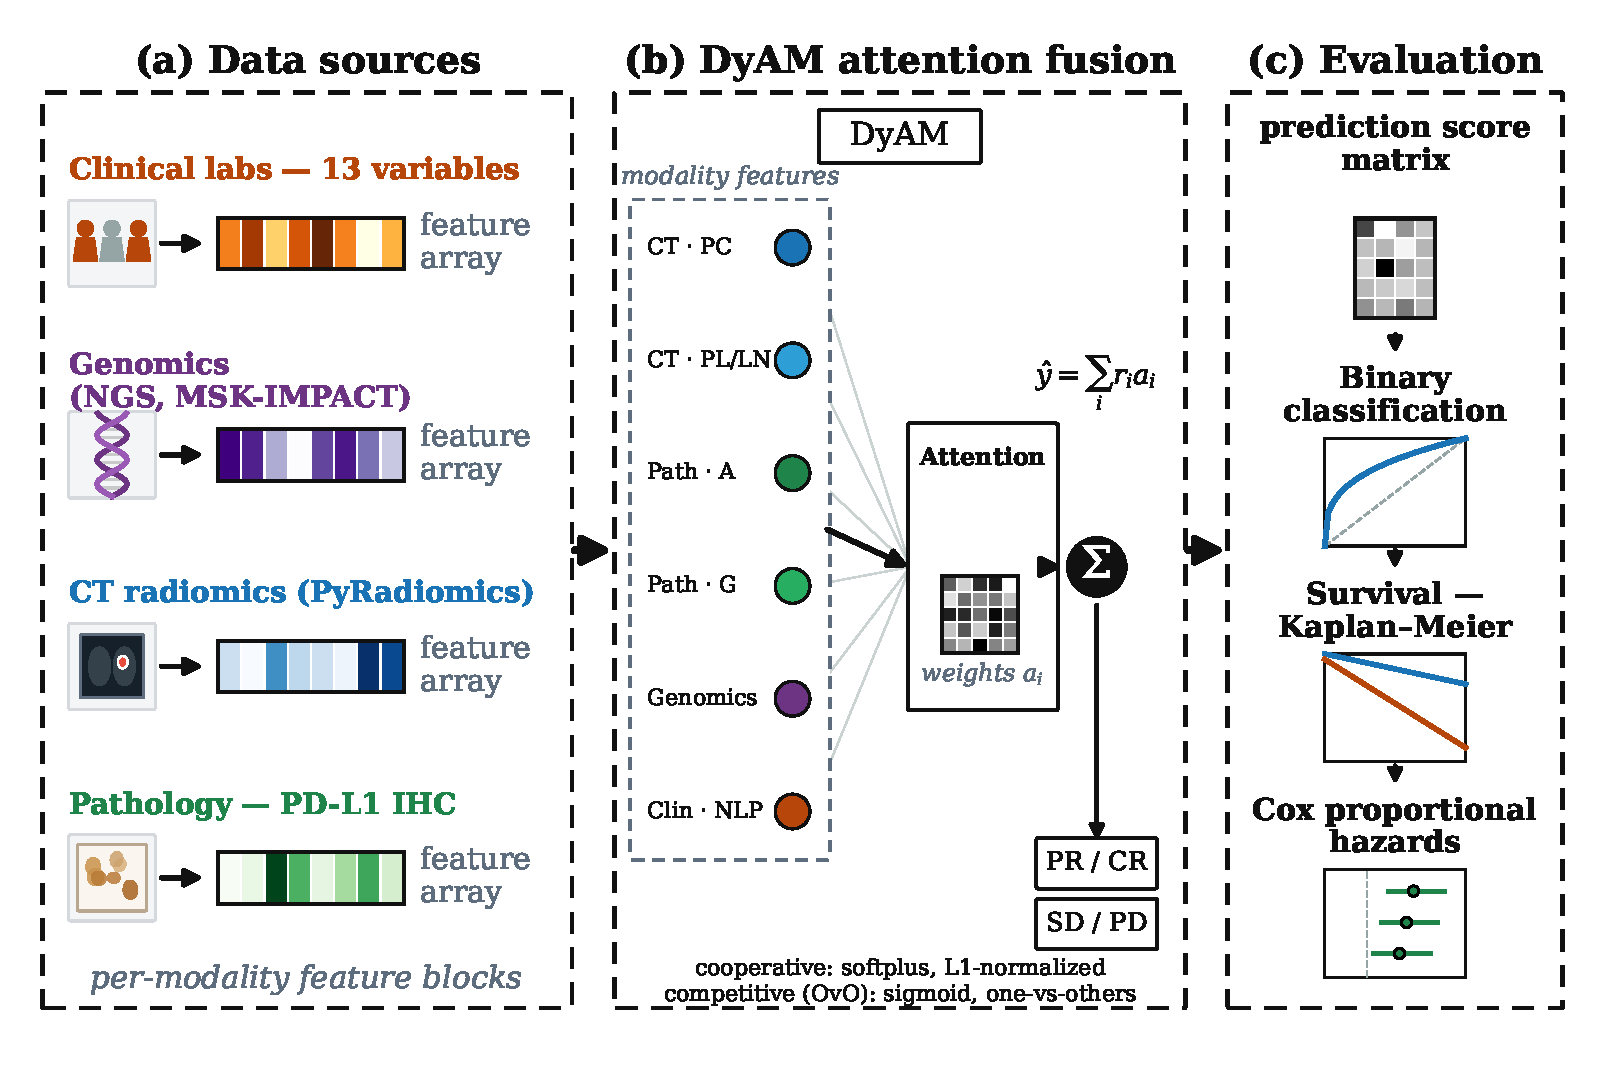
\includegraphics[width=\textwidth]{figures/fig1_overview_demo.pdf}
  \caption{Study overview. (A) The discovery cohort ($n = 247$) and two
    validation cohorts (radiomics-evaluable, $n = 50$; pathology-evaluable,
    $n = 71$) provide six data sources: CT radiomics (modelled separately
    per lesion site: PC, PL, LN), pathology image texture (IHC-A or IHC-G),
    tumour genomics, PD-L1~TPS, and structured clinical variables, giving up
    to seven input modalities per model. (B) The DyAM architecture computes a
    per-modality risk score and combines modalities using either cooperative
    (\texttt{AttentionMatrix}) or competitive one-vs-others
    (\texttt{AttentionMatrixOvO}) attention to produce a fused risk
    prediction $\hat{y}$. (C) Models are evaluated on both binary response
    classification (AUC-ROC with DeLong 95\% CI) and survival endpoints
    (Harrell's C-index, multivariate Cox hazard ratios, and Kaplan--Meier
    log-rank stratification).}
  \label{fig:overview}
\end{figure}

%% ═══════════════════════════════════════════════════════════════════════════
%% B2 — Data Modalities
%% ═══════════════════════════════════════════════════════════════════════════

\subsection{Data Modalities}
\label{sec:modalities}

Six data sources were assembled for each patient
(Table~\ref{tab:modalities}).
Because CT radiomics is modelled separately per lesion site (PC, PL, LN) and
the two pathology feature sets (IHC-A, IHC-G) are used as alternative arms
rather than jointly, a single model receives up to seven input modalities.
CT radiomics features were extracted from baseline scans using
PyRadiomics \cite{vanGriethuysen2017}, following the preprocessing of
\cite{Vanguri2022}, at 1.0~mm isotropic spacing with a window of
$[{-1350}, 250]$~HU, yielding 1{,}688 features per lesion type.
Lesions were categorised by anatomical site:
primary tumour (PC), pleural lesion (PL), and lymph node (LN).
Up to three lesions per site were included, ranked by volume.
Pathology features were derived from PD-L1 immunohistochemistry (IHC) slides:
\emph{IHC-A} comprised 18 pixel-intensity aggregation features
(area, mean intensity, percentiles), while
\emph{IHC-G} comprised 150 grey-level co-occurrence matrix (GLCM)
texture features across six aggregation levels \cite{Vanguri2022}.
Genomic features (11 variables) included tumour mutational burden (TMB) and
the status of eight driver mutations and amplifications derived from
MSK-IMPACT targeted next-generation sequencing (NGS) \cite{Cheng2015}.
The PD-L1 tumour proportion score (TPS) was obtained from clinical
pathology reports (range 0--100\%).
Clinical laboratory features comprised 13 variables:
age, smoking pack-years, Eastern Cooperative Oncology Group (ECOG)
performance status, serum albumin,
derived neutrophil-to-lymphocyte ratio (dNLR), initial tumour burden,
brain and liver metastasis status, line of therapy, combination therapy,
primary lung site, prior PD-L1 therapy, and adenocarcinoma histology.

For radiomics modalities, features with an intraclass correlation coefficient
(ICC) below 0.15 across test--retest perturbation scans were removed
(robustness filter), and features with a $z$-score exceeding 6 in any patient
were flagged as outliers and excluded.
All modalities except the NLP embedding (Section~\ref{sec:nlp}) were
standardised with \texttt{RobustScaler} (median centring, IQR scaling).
Missing modalities were handled via a binary indicator mask
$\mathbf{m} \in \{0,1\}^N$; masked modalities contribute zero attention and
zero risk to the fused prediction (Section~\ref{sec:model}).

\begin{table}[H]
\caption{Summary of data modalities used in this study.
  All feature counts are post-selection (after ICC and outlier filtering
  for radiomics).
  NLP, natural language processing; GLCM, grey-level co-occurrence matrix;
  IHC, immunohistochemistry; NGS, next-generation sequencing;
  TPS, tumour proportion score.}
\label{tab:modalities}
\small
\begin{tabular}{@{}p{2.3cm}p{2.7cm}p{1.2cm}p{4.1cm}@{}}
\toprule
\textbf{Modality} & \textbf{Source} & \textbf{Features} & \textbf{Clinical meaning} \\
\midrule
CT Radiomics (PC, PL, LN) & PyRadiomics & $\leq$1{,}688 & Tumour shape, size, and texture from baseline CT \\
Pathology IHC-A            & PD-L1 IHC slides & 18  & Pixel-intensity aggregation of PD-L1 expression \\
Pathology IHC-G            & PD-L1 IHC slides & 150 & GLCM texture of PD-L1 signal \\
Genomics                   & MSK-IMPACT & 11 & TMB + driver mutation/amplification status \\
PD-L1 TPS                  & Pathology report  & 1  & Tumour proportion score (0--100\%) \\
Clinical labs              & EHR               & 13 & Demographics, performance status, labs \\
\textbf{NLP embedding} (new) & \texttt{all-MiniLM-L6-v2} & 384 & Sentence embedding of clinical lab text \\
\textbf{NLP-PCA16} (new)   & PCA of NLP        & 16  & PCA-compressed NLP (approx.\ 94\% variance) \\
\bottomrule
\end{tabular}
\end{table}

%% ═══════════════════════════════════════════════════════════════════════════
%% B3 — NLP Clinical Embedding
%% ═══════════════════════════════════════════════════════════════════════════

\subsection{NLP Encoding of Tabular Clinical Features}
\label{sec:nlp}

Standard encoding of clinical variables as a 13-dimensional numeric vector
treats each feature independently and loses contextual relationships between
variables (e.g., an elderly patient with low albumin and ECOG~2 implies a
different prognosis than the same values in isolation).
To capture inter-feature context, we converted each patient's clinical
profile into an English-language sentence and extracted a dense semantic
embedding, as illustrated in Figure~\ref{fig:nlp_pipeline}.

\paragraph{Text prompt construction.}
For each patient, the 13 clinical variables were formatted into a structured
natural-language sentence, for example:
\textit{``The patient is a 69-year-old. Smoking history in pack-years is 48.0.
ECOG performance status is 1.0. Blood albumin concentration is 4.00.
Derived neutrophil-to-lymphocyte ratio (dNLR) is 2.40.
Initial tumor burden stands at 52.00.
The patient is diagnosed with adenocarcinoma at the lung site.
Metastatic status: without brain metastasis and without liver metastasis.
Currently undergoing therapy line 2, utilizing combination therapy.
The patient received prior PD-L1 immunotherapy.''}
Binary variables were expanded to descriptive phrases to exploit the
pretrained vocabulary of the encoder.
The full prompt template is provided in Supplementary Note~S1.

\paragraph{Sentence encoder.}
Prompts were encoded with
\texttt{sentence-transformers/all-MiniLM-L6-v2} \cite{Reimers2019,Wang2020MiniLM},
a 6-layer transformer distilled for semantic sentence similarity and
trained on over one billion sentence pairs.
Each patient was represented as a 384-dimensional L2-normalised vector.
No fine-tuning was performed; the model was applied in zero-shot transfer.
We compared this general-purpose encoder against the domain-specific
\texttt{Bio\_ClinicalBERT} \cite{Alsentzer2019};
the domain-specific model performed inferiorly
($\Delta\text{AUC} = -0.012$ versus MiniLM-L6-v2 in the IHC-A arm),
consistent with its design for masked language modelling
rather than sentence-similarity tasks (Supplementary Note~S2).

\paragraph{Dimensionality reduction.}
Principal component analysis (PCA) was applied to the 384-dimensional embeddings,
retaining the top 16 components ($\approx$94\% of variance explained;
Supplementary Figure~S1).
Both the raw 384-dimensional (\emph{NLP raw}) and PCA-compressed
16-dimensional (\emph{NLP-PCA16}) variants were evaluated.
Crucially, the NLP modality was passed to the model with the RobustScaler
disabled (\texttt{no\_scale=True}), as the embeddings are already L2-normalised
and scaling would distort the cosine-similarity geometry of the embedding space.

\begin{figure}[H]
  \centering
  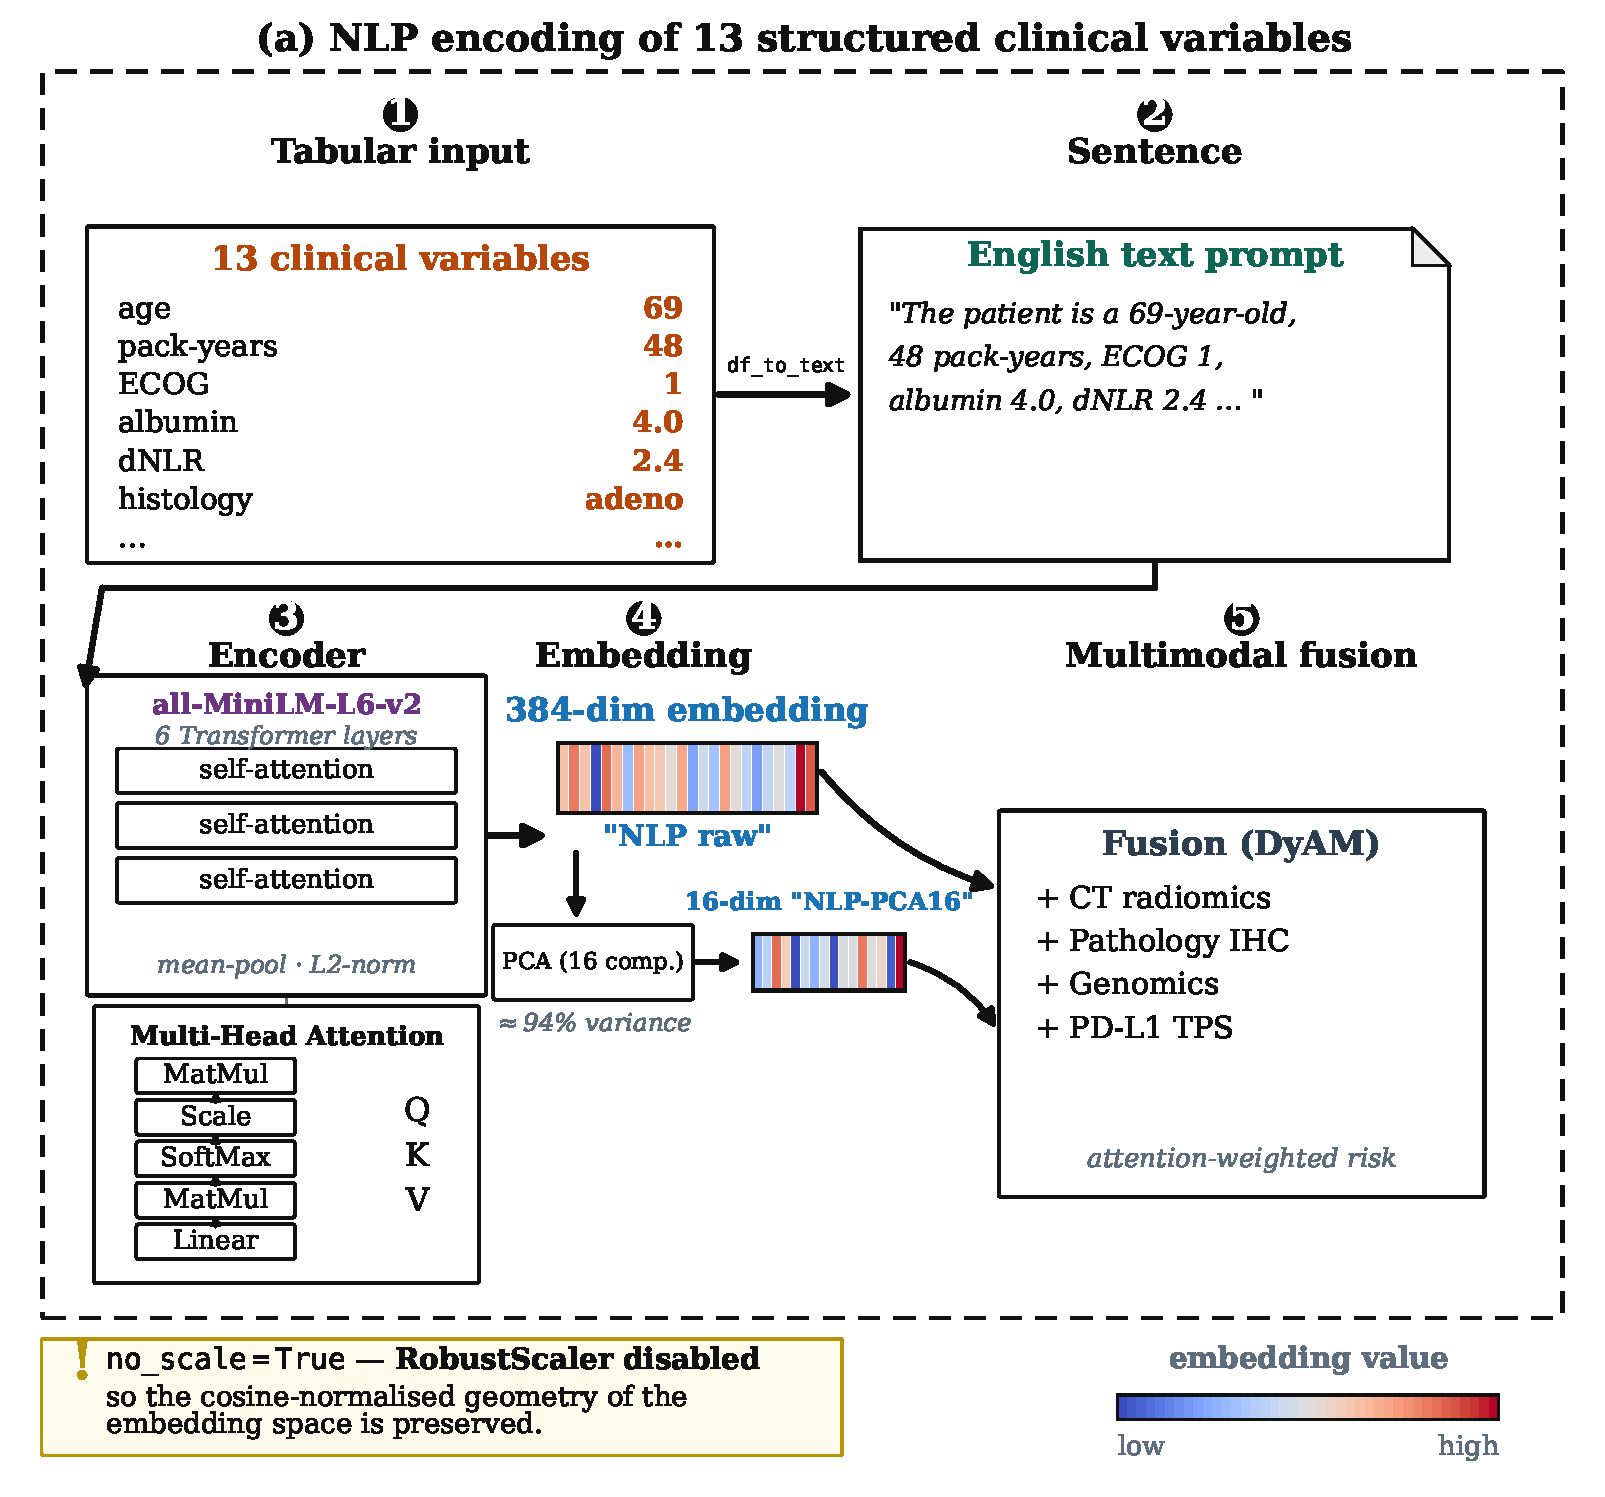
\includegraphics[width=\textwidth]{figures/fig2_nlp_pipeline_demo.pdf}
  \caption{NLP-based encoding of structured clinical features. Thirteen
    numeric clinical variables per patient are converted into a
    natural-language sentence describing the patient's clinical profile
    (example shown), which is then encoded into a 384-dimensional embedding
    using a pretrained sentence transformer (all-MiniLM-L6-v2). The
    384-dimensional embedding (``NLP raw'') is used directly, or further
    reduced to 16 dimensions via PCA (``NLP-PCA16'', retaining
    $\approx$94\% of variance) prior to fusion with other modalities.
    \texttt{no\_scale=True} is applied to NLP embeddings to preserve their
    cosine-normalised geometry.}
  \label{fig:nlp_pipeline}
\end{figure}

%% ═══════════════════════════════════════════════════════════════════════════
%% B4 — Model Architecture
%% ═══════════════════════════════════════════════════════════════════════════

\subsection{Model Architecture}
\label{sec:model}

\paragraph{Dynamic Attention Multimodal (DyAM) model.}
The base model, DyAM \cite{Vanguri2022}, fuses $N$ modalities through
per-modality risk scores and a learned attention mechanism, in the spirit of
attention-based architectures broadly \cite{Vaswani2017}.
Let $\mathbf{x}_i \in \mathbb{R}^{d_i}$ denote the feature vector of
modality~$i$ after optional RobustScaling.
A scalar risk score is computed as:
%
\begin{equation}
  r_i = \tanh\!\left(\mathbf{W}_{\mathrm{r},i}^{\top} \mathbf{x}_i\right),
  \label{eq:risk}
\end{equation}
%
where $\mathbf{W}_{\mathrm{r},i} \in \mathbb{R}^{d_i}$ are learnable weights.
An attention score is produced by an $N \times N$ grid of linear layers
with softplus activation, $\ell_2$-normalised by the modality vector norm:
%
\begin{equation}
  s_i = \frac{\mathrm{softplus}\!\left(\mathbf{W}_{\mathrm{a},ij}^{\top}
        \mathbf{x}_i\right)}{\left\|\mathbf{x}_i\right\|_2}.
  \label{eq:attn_s}
\end{equation}
%
Attention weights are obtained by L1 normalisation across modalities:
%
\begin{equation}
  a_i = \frac{s_i}{\displaystyle\sum_{j=1}^{N} s_j}.
  \label{eq:attn_a}
\end{equation}

\paragraph{OvO competitive attention.}
We propose an alternative attention mechanism inspired by
one-versus-others (OvO) classification \cite{Rifkin2004},
in which each modality \emph{competes} against the mean score of
all remaining modalities rather than sharing a fixed budget.
The mean score of the $N-1$ competing modalities is:
%
\begin{equation}
  \mu_{-i} = \frac{1}{N-1} \sum_{j \neq i} s_j,
  \label{eq:ovo_mu}
\end{equation}
%
and the OvO attention score is:
%
\begin{equation}
  \mathrm{ovo}_i = \sigma\!\left(s_i - \mu_{-i}\right),
  \qquad \sigma(z) = (1+e^{-z})^{-1}.
  \label{eq:ovo}
\end{equation}
%
The sigmoid function yields an independent probability that modality~$i$
outperforms the others, rather than a jointly normalised score.
After applying the binary missingness mask $m_i \in \{0,1\}$, the weights
are L1-normalised: $a_i = \mathrm{ovo}_i \cdot m_i \big/
\sum_j \mathrm{ovo}_j \cdot m_j$.
The two attention mechanisms are contrasted schematically in
Figure~\ref{fig:attention_arch}.

\paragraph{Fused prediction and training.}
For both variants, the final risk prediction is:
%
\begin{equation}
  \hat{y} = \sum_{i=1}^{N} r_i \cdot a_i.
  \label{eq:output}
\end{equation}
%
\begin{figure}[H]
  \centering
  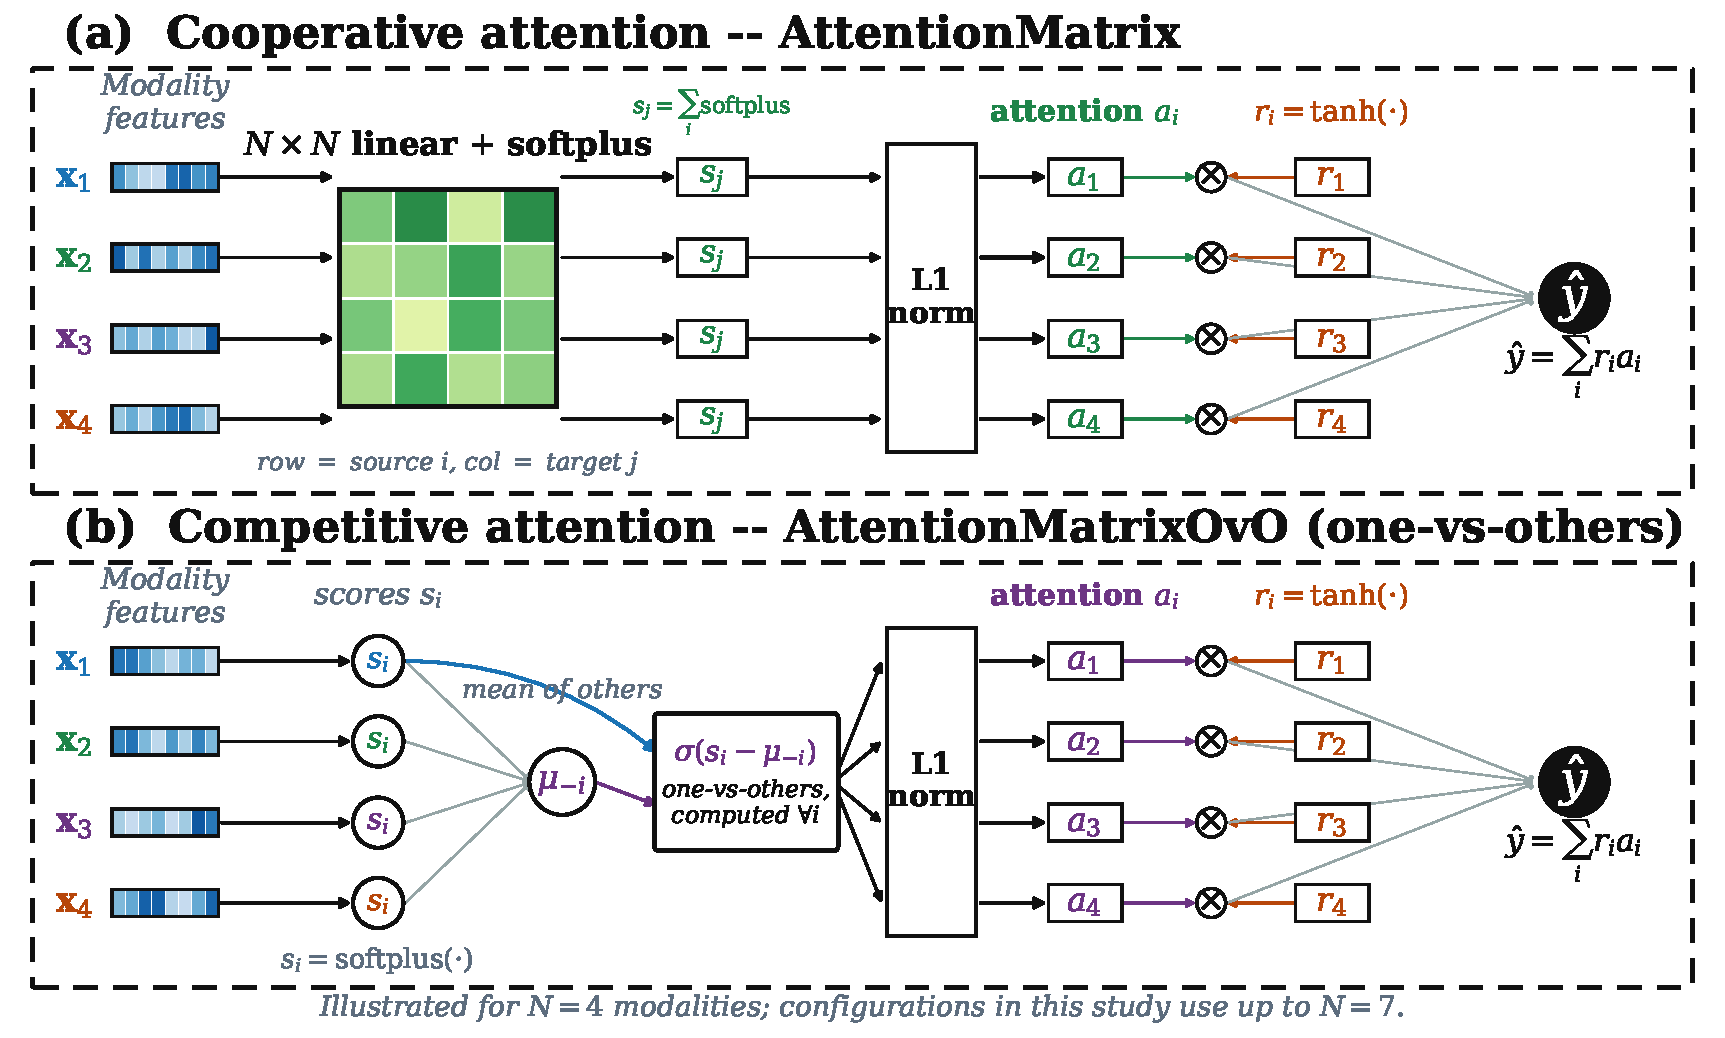
\includegraphics[width=\textwidth]{figures/fig_attention_arch_demo.pdf}
  \caption{Architecture of the two attention mechanisms. Both variants
    compute a per-modality risk score $r_i = \tanh(\mathbf{W}_{r,i}^{\top}
    \mathbf{x}_i)$ (Equation~\ref{eq:risk}) and produce the fused prediction
    $\hat{y} = \sum_i r_i a_i$ (Equation~\ref{eq:output}); they differ only in
    how the attention weights $a_i$ are obtained.
    (A)~\emph{Cooperative} attention (\texttt{AttentionMatrix}): an
    $N\times N$ grid of linear layers with softplus activation produces
    pairwise scores that are column-summed into $s_j$
    (Equation~\ref{eq:attn_s}) and L1-normalised so that the modalities
    share a fixed attention budget (Equation~\ref{eq:attn_a}).
    (B)~\emph{Competitive} one-vs-others attention
    (\texttt{AttentionMatrixOvO}): each modality produces a single score
    $s_i$ that is compared against the mean score of the remaining
    modalities $\mu_{-i}$ through a sigmoid, $\sigma(s_i - \mu_{-i})$
    (Equations~\ref{eq:ovo_mu}--\ref{eq:ovo}), yielding an independent
    competitive weight before L1 normalisation.
    Heatmap bars denote modality feature vectors; the diagram is drawn for
    $N = 4$ modalities for clarity.}
  \label{fig:attention_arch}
\end{figure}

The model was trained with binary cross-entropy loss
(\texttt{BCEWithLogitsLoss}) with automatic inverse-frequency class
weighting to address the $\approx$1:3 class imbalance,
an $\ell_2$ penalty on the weights (coefficient $\alpha = 0.001$);
the attention-norm penalty was disabled ($\beta = 0$).
The Adam optimiser was used with a learning rate of 0.01 for 125 epochs.
All experiments used 10-fold cross-validation (shuffled, not stratified) on the
discovery cohort; predictions were pooled across held-out folds for
AUC computation.

%% ═══════════════════════════════════════════════════════════════════════════
%% B5 — Statistical Analysis
%% ═══════════════════════════════════════════════════════════════════════════

\subsection{Statistical Analysis and Evaluation}
\label{sec:stats}

\paragraph{Discriminative performance.}
Area under the receiver operating characteristic curve (AUC-ROC) was
computed on pooled out-of-fold predictions from 10-fold cross-validation.
Ninety-five percent confidence intervals (CIs) were estimated using the
DeLong structural components method \cite{DeLong1988}.
All results come from a single 10-fold cross-validation partition (seed~42, natural patient order, the
protocol of the original publication). Differences between models are reported as the difference in AUC and the
number of configurations favouring each model. Because the cohort is small, hypothesis tests were not
used to claim that one model is superior; DeLong intervals are reported for single AUC values.

\paragraph{Survival analysis.}
Harrell's concordance index (C-index) \cite{Harrell1996} was computed from
pooled out-of-fold risk scores against PFS, from the same partition.
Multivariate Cox proportional hazards regression was fitted with the
DyAM risk score as the primary predictor, adjusted for five clinical
covariates: age, ECOG performance status, serum albumin, dNLR, and
liver metastasis status; hazard ratios are per unit of risk score.
Time-dependent AUC (6, 12 and 18~months; cumulative/dynamic estimator
\cite{Uno2007,Hung2010}) was computed from the same partition
(\texttt{scikit-survival}~0.28 with \texttt{numpy}~2.5.4 in a separate environment, from the stored out-of-fold
risk scores).

\paragraph{Kaplan--Meier survival stratification.}
Patients were dichotomised at the median risk score, and PFS curves for the
two groups were compared with the log-rank test.
The log-rank $\chi^2$ is reported with $\chi^2 > 3.84$ ($p < 0.05$) and
$\chi^2 > 7.88$ ($p < 0.005$) as reference values.

\paragraph{Software.}
All numerical results in Tables~\ref{tab:ovo_all21}--\ref{tab:km} were computed in one pinned environment
(Linux under WSL2, Ubuntu~22.04; Python~3.8.15, PyTorch~1.8.1 (CPU), \texttt{scikit-learn}~0.24.2,
\texttt{scipy}~1.6.3, \texttt{numpy}~1.20.3, \texttt{pandas}~1.2.5, and \texttt{lifelines}~0.26.0 for
Kaplan--Meier, Cox regression and the C-index). In this environment the original DyAM code reproduced the
single-partition AUC of the original publication at its primary benchmark (0.798) to within one patient pair.
The same code and library versions on another operating system gave AUCs that differed in the second or
third decimal place, so results were never compared across platforms; the radiomics feature selection used
the original procedure, without removal of degenerate columns. The sentence-encoder embeddings (MiniLM-L6-v2
and Bio\_ClinicalBERT) were computed once in a separate environment and cached, and time-dependent AUC was
computed from the stored out-of-fold risk scores with \texttt{scikit-survival}~0.28 (\texttt{numpy}~2.5.4).

%% sections/results.tex — single-partition version
%% NOTE: all numbers in the tables are generated by make_tables_single.py
\section{Results}
\label{sec:results}

All results are from a single 10-fold cross-validation partition of the 247-patient discovery cohort
(natural patient order, the evaluation protocol of the original DyAM publication). Because one partition
can favour any model by chance, differences of the size reported below are described by direction and
magnitude, and the confidence intervals reflect patient sampling only.

\subsection{Multimodal Fusion Outperforms Single-Modality Baselines}
\label{sec:baselines}

Within the DyAM framework, models restricted to a single data source achieved AUC values of
$0.615$ (TMB), $0.606$ (pathology IHC-A), $0.701$ (CT radiomics), $0.676$ (genomics), and
$0.708$ (PD-L1~TPS) on the discovery cohort.
PD-L1~TPS was the strongest individual predictor among the biomarkers of routine clinical use,
although CT radiomics was comparable.

Fusing four data sources (CT radiomics, pathology IHC-A, genomics, and PD-L1~TPS) raised the AUC to
$0.798$ under the cooperative attention of the original framework, exceeding the best single source by
$0.090$~AUC; with IHC-G in place of IHC-A the four-source model reached $0.783$ (95\% CI 0.714--0.853),
and adding NLP-encoded clinical variables raised the latter to $0.803$ (0.738--0.868) (Table~\ref{tab:ovo_all21}).
Multimodal fusion is therefore the primary driver of predictive performance in this cohort, with no
individual source approaching the discrimination of the fused model.

%% ═══════════════════════════════════════════════════════════════════════════
%% B8 — NLP AUC Analysis
%% ═══════════════════════════════════════════════════════════════════════════

\subsection{NLP Encoding Improves AUC over Numeric Clinical Labs}
\label{sec:nlp_auc}

Seven clinical-encoding variants were evaluated under the DyAM architecture in two pathology
arms (IHC-A: seven variants; IHC-G: four variants)
(Tables~\ref{tab:auc_ihca} and \ref{tab:auc_ihcg}; Figure~\ref{fig:auc_comparison}).
Relative to numeric labs, the NLP raw (384-dimensional) encoding raised the AUC by
$+0.018$ in the IHC-A arm ($0.786$ vs.\ $0.768$) and by $+0.019$ in the IHC-G arm
($0.812$ vs.\ $0.792$); the PCA-compressed NLP variant gave $+0.015$ and $+0.013$.
These differences are within the width of the confidence intervals ($\approx 0.14$), so they should be
read as a consistent direction of modest size.
The same advantage over numeric labs was present in the 21-configuration analysis for both
attention mechanisms: in the two seven-source configurations that contain labs
(Table~\ref{tab:ovo_all21}, rows 20 and 21), replacing labs by the NLP encoding raised the
AUC from $0.753$ to $0.772$ and from $0.781$ to $0.803$ for DyAM, and from $0.749$ to
$0.782$ and from $0.794$ to $0.824$ for OvO.

\emph{Comparison with no clinical information.}
The NLP raw encoding was above the no-clinical baseline by $+0.014$ in both arms
(IHC-A: $0.786$ vs.\ $0.772$; IHC-G: $0.812$ vs.\ $0.797$), whereas numeric labs were slightly below it
($-0.004$ and $-0.005$).
At BM2 of the 21-configuration analysis NLP was above BM1 (the configuration without clinical
variables) by $+0.020$ for DyAM and $+0.024$ for OvO.
These gains are small relative to the confidence intervals, so we base the main claim on NLP versus
numeric labs and regard the benefit of NLP encoding over omitting clinical variables as small and not
established in this cohort.

\emph{Domain-specific versus general-purpose encoder.}
Bio\_ClinicalBERT \cite{Alsentzer2019}, PCA-compressed to 16 dimensions,
reached $0.770$ in the IHC-A arm, below MiniLM-L6-v2 with the same compression
($0.784$; $\Delta\text{AUC} = -0.014$) and equal to numeric labs ($0.768$) and slightly
below the no-clinical baseline ($0.772$; Supplementary Note~S2),
consistent with its pretraining objective of masked language modelling
on clinical notes rather than semantic sentence similarity.

\emph{Combined encoding.}
Concatenating numeric labs and the NLP encoding as separate sources
(8 sources in total) did not improve on the NLP encoding alone
(IHC-A: $0.784$ for NLP-PCA16 alone vs.\ $0.767$ for labs + NLP-PCA16),
and with $n/N = 247/8 \approx 31$ the attention weights are poorly determined.
NLP encoding is therefore used as a \emph{replacement} for,
rather than an addition to, numeric clinical features.

%% tables/table2_auc_ihca.tex  (GENERATED by make_tables_single.py - do not edit by hand)
\begin{table}[H]
\caption{AUC comparison across clinical encoding strategies --- IHC-A arm. All models use the DyAM
  architecture with CT radiomics (PC, PL, LN), pathology IHC-A, genomics, and PD-L1~TPS as base modalities;
  clinical encoding is the varied factor. Values are the AUC of a single 10-fold cross-validation partition
  ($n = 247$) with the DeLong 95\% confidence interval. $\Delta$AUC is the difference relative to the
  no-clinical baseline and to numeric labs. n/a, not applicable. NLP, natural language processing;
  PCA, principal component analysis.}
\label{tab:auc_ihca}
\begin{tabular}{lccc}
\toprule
\textbf{Model} & \textbf{AUC [95\% CI]} & \boldmath{$\Delta$}\textbf{ vs no clinical} & \boldmath{$\Delta$}\textbf{ vs labs} \\
\midrule
No clinical (baseline)         & 0.772 [0.707, 0.838] & (ref) & n/a \\
+ Labs (13-dim numeric)        & 0.768 [0.701, 0.836] & $-0.004$ & n/a \\
+ NLP raw (384-dim)            & 0.786 [0.725, 0.847] & $+0.014$ & $+0.018$ \\
+ NLP-PCA16 (16-dim)           & 0.784 [0.722, 0.845] & $+0.012$ & $+0.015$ \\
+ Labs + NLP (combined)        & 0.758 [0.690, 0.826] & $-0.014$ & $-0.010$ \\
+ Labs + NLP-PCA16 (combined)  & 0.767 [0.700, 0.834] & $-0.005$ & $-0.001$ \\
+ BioClinBERT-PCA16            & 0.769 [0.705, 0.834] & $-0.003$ & $+0.001$ \\
\bottomrule
\end{tabular}
\end{table}

%% tables/table3_auc_ihcg.tex  (GENERATED by make_tables_single.py - do not edit by hand)
\begin{table}[H]
\caption{AUC comparison across clinical encoding strategies --- IHC-G arm. All models use the DyAM
  architecture with CT radiomics (PC, PL, LN), pathology IHC-G, genomics, and PD-L1~TPS as base modalities;
  clinical encoding is the varied factor. Values are the AUC of a single 10-fold cross-validation partition
  ($n = 247$) with the DeLong 95\% confidence interval. $\Delta$AUC is the difference relative to the
  no-clinical baseline and to numeric labs. n/a, not applicable. NLP, natural language processing;
  PCA, principal component analysis.}
\label{tab:auc_ihcg}
\begin{tabular}{lccc}
\toprule
\textbf{Model} & \textbf{AUC [95\% CI]} & \boldmath{$\Delta$}\textbf{ vs no clinical} & \boldmath{$\Delta$}\textbf{ vs labs} \\
\midrule
No clinical (baseline)         & 0.797 [0.731, 0.863] & (ref) & n/a \\
+ Labs (13-dim numeric)        & 0.792 [0.726, 0.859] & $-0.005$ & n/a \\
+ NLP raw (384-dim)            & 0.812 [0.753, 0.871] & $+0.014$ & $+0.019$ \\
+ NLP-PCA16 (16-dim)           & 0.805 [0.745, 0.866] & $+0.008$ & $+0.013$ \\
\bottomrule
\end{tabular}
\end{table}


\begin{figure}[H]
  \centering
  \subfloat[IHC-A arm (7 variants)\label{fig:auc_ihca}]{%
    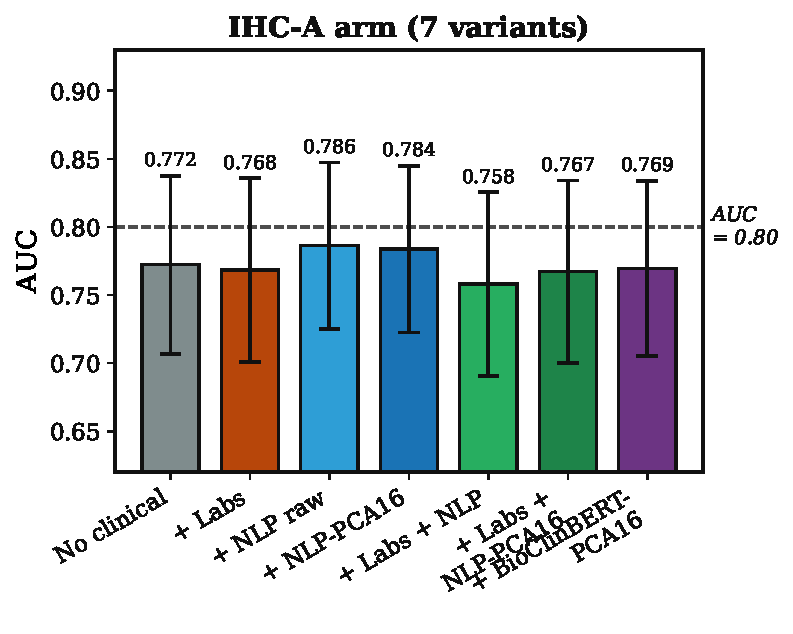
\includegraphics[width=0.48\textwidth]{figures/fig3a_auc_ihca_demo.pdf}}
  \hfill
  \subfloat[IHC-G arm (4 variants)\label{fig:auc_ihcg}]{%
    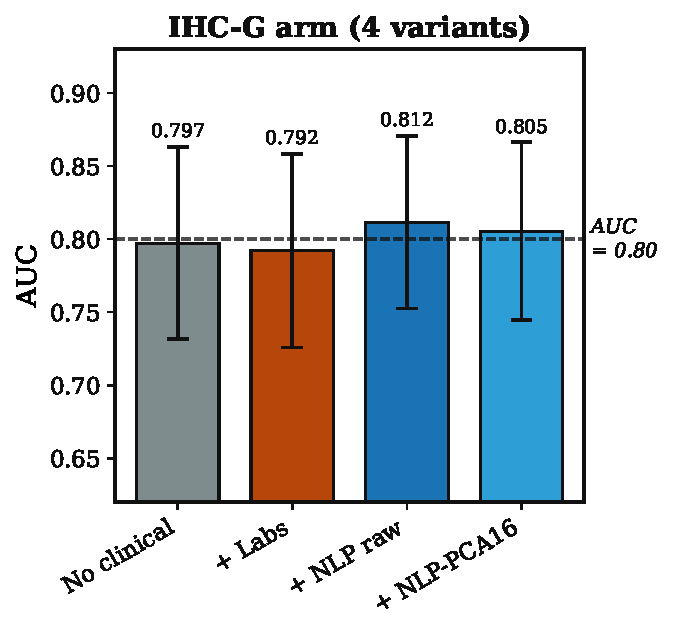
\includegraphics[width=0.48\textwidth]{figures/fig3b_auc_ihcg_demo.pdf}}
  \caption{AUC comparison across clinical encoding strategies for
    (\textbf{A}) the IHC-A arm and (\textbf{B}) the IHC-G arm. Bars show
    the AUC of a single 10-fold cross-validation partition ($n = 247$); error
    bars denote the DeLong 95\% confidence interval. The
    dashed horizontal line at AUC~$=0.80$ marks the conventional threshold
    for clinically useful discrimination.}
  \label{fig:auc_comparison}
\end{figure}

\subsection{OvO Competitive Attention with NLP Encoding Gives the Highest Fusion AUC with a Simpler Parameterization}
\label{sec:ovo}

We compared the OvO attention variant with the original cooperative attention across the 21 modality
combinations of the primary paper-matched configuration set, without and with the NLP-clinical encoding
of Section~\ref{sec:nlp_auc} (Table~\ref{tab:ovo_all21}).
Because a cohort of 247 patients cannot support reliable hypothesis tests of differences of this size,
we report the difference in AUC and the number of configurations favouring each model; we do not use
significance testing to claim superiority.

Without NLP, the largest gains for OvO over the cooperative model were for TMB+PDL1 ($\Delta\text{AUC} = +6.29\%$, AUC 0.699 vs.\ 0.636) and PDL1+Gen
($+2.27\%$, 0.716 vs.\ 0.693; Table~\ref{tab:ovo}); the cooperative model was higher for IHC-G+Gen ($-3.27\%$)
and Rad+IHC-A+Gen+PDL1 ($-3.03\%$).
At the primary benchmark (Rad+IHC-G+Gen+PDL1, BM1), OvO reached an AUC of $0.801$ (95\% CI 0.735--0.866)
versus $0.783$ (0.714--0.853) for the cooperative model ($\Delta\text{AUC} = +0.017$).

Only the two configurations that contain numeric labs (rows 20 and 21) have an NLP counterpart in
Table~\ref{tab:ovo_all21}, because the NLP encoding replaces the labs source; the remaining configurations contain no
clinical information, so their +NLP entries simply repeat the values without NLP.
In the labs-replaced configuration of BM2 (Rad+IHC-G+Gen+PDL1 with NLP), DyAM+NLP reached $0.803$ (0.738--0.868) and
OvO+NLP $0.824$ (0.765--0.883) ($\Delta = +0.021$); the intervals overlap almost completely.
Relative to BM1, which has the same sources without any clinical variable, the NLP gain was $+0.020$ for DyAM and
$+0.024$ for OvO.
OvO+NLP reached the highest AUC in this study ($0.824$), against $0.803$ for DyAM+NLP and $0.798$ for
the cooperative model without NLP (Rad+IHC-A+Gen+PDL1, the primary result of the original publication, which
this evaluation reproduced).

OvO's potential advantage is plausibly one of parameter economy: with the 384-dimensional NLP source
in the BM2 configuration, the cooperative model has 4{,}969 trainable parameters against 1{,}242 for OvO.
We did not test this explanation directly; for example, we did not shrink the cooperative attention matrix
to see whether the gap closes.
Table~\ref{tab:ovo} gives the largest single-configuration differences and Table~\ref{tab:ovo_all21} the AUC
of both attention mechanisms, with and without NLP, across all 21 configurations.

\begin{table}[H]
\caption{Largest differences between OvO competitive attention and original cooperative attention among the
  21 configurations, from a single 10-fold partition.
  $\Delta$AUC is computed as OvO minus Original.
  The upper block lists configurations in which OvO was higher, the lower block those in which the original was higher.
  Bold denotes the higher AUC for each row.
  Differences from one partition can favour either model by chance.
  Gen, genomics; Rad, CT radiomics; IHC-A/G, immunohistochemistry variants;
  PDL1, PD-L1 TPS score.}
\label{tab:ovo}
\centering
\footnotesize
\begin{tabular}{@{}lccc@{}}
\toprule
Configuration & Orig. & OvO & $\Delta$ \\
\midrule
TMB+PDL1                & 0.636 & \textbf{0.699} & +6.29\% \\
PDL1+Gen                & 0.693 & \textbf{0.716} & +2.27\% \\
Rad+IHC-G+Gen+PDL1      & 0.783 & \textbf{0.801} & +1.71\% \\
Rad+IHC-G+Gen+PDL1+Labs & 0.781 & \textbf{0.794} & +1.22\% \\
Rad+IHC-A+Gen+TMB+PDL1  & 0.778 & \textbf{0.780} & +0.24\% \\
\midrule
Rad+IHC-G               & \textbf{0.713} & 0.702 & $-1.10\%$ \\
Rad-LU                  & \textbf{0.699} & 0.684 & $-1.53\%$ \\
Rad+IHC-A+MutAmp        & \textbf{0.782} & 0.767 & $-1.54\%$ \\
Rad+IHC-A+Gen+PDL1      & \textbf{0.798} & 0.768 & $-3.03\%$ \\
IHC-G+Gen               & \textbf{0.756} & 0.723 & $-3.27\%$ \\
\bottomrule
\end{tabular}
\end{table}

%% tables/table_ovo_all21.tex  (GENERATED by make_tables_single.py - do not edit by hand)
\begin{table}[H]
\centering
\caption{AUC across all 21 paper-matched modality combinations for cooperative attention (DyAM) and OvO
  competitive attention, each without and with NLP-clinical encoding, from a single 10-fold
  cross-validation partition (natural patient order, the protocol of the original DyAM publication;
  $n = 247$). $k$ is the number of fused input sources (CT radiomics contributes one source per lesion
  site). For $k = 1$ OvO reduces algebraically to the
  cooperative formulation, hence the identical values. Configurations 8, 11, 18 and 21 are the primary
  benchmarks BM4, BM3, BM1 and BM2. The NLP encoding replaces the numeric labs source, so only the two configurations that contain labs (20 and 21) differ between the models with and without NLP; the other configurations contain no clinical source, and their +NLP values repeat those of the models without NLP (not in bold). Bold marks the highest value in each row.}
\label{tab:ovo_all21}
\footnotesize
\begin{tabular}{@{}rlcrrrr@{}}
\toprule
\# & Configuration & $k$ & DyAM & OvO & DyAM+NLP & OvO+NLP \\
\midrule
1  & TMB                              & 1 & \textbf{0.615} & \textbf{0.615} & 0.615 & 0.615 \\
2  & PDL1                             & 1 & \textbf{0.708} & \textbf{0.708} & 0.708 & 0.708 \\
3  & IHC-A                            & 1 & \textbf{0.606} & \textbf{0.606} & 0.606 & 0.606 \\
4  & Gen                              & 1 & \textbf{0.676} & \textbf{0.676} & 0.676 & 0.676 \\
5  & Rad                              & 3 & \textbf{0.701} & 0.700 & 0.701 & 0.700 \\
6  & Rad-LU                           & 4 & \textbf{0.699} & 0.684 & 0.699 & 0.684 \\
7  & TMB+PDL1                         & 2 & 0.636 & \textbf{0.699} & 0.636 & 0.699 \\
8  & PDL1+Gen (BM4)                   & 2 & 0.693 & \textbf{0.716} & 0.693 & 0.716 \\
9  & Rad+IHC-A                        & 4 & \textbf{0.681} & 0.672 & 0.681 & 0.672 \\
10 & Rad+IHC-G                        & 4 & \textbf{0.713} & 0.702 & 0.713 & 0.702 \\
11 & Rad+Gen (BM3)                    & 4 & \textbf{0.759} & 0.755 & 0.759 & 0.755 \\
12 & IHC-A+Gen                        & 2 & 0.715 & \textbf{0.716} & 0.715 & 0.716 \\
13 & IHC-G+Gen                        & 2 & \textbf{0.756} & 0.723 & 0.756 & 0.723 \\
14 & Rad+IHC-A+Gen                    & 5 & \textbf{0.754} & 0.748 & 0.754 & 0.748 \\
15 & Rad+IHC-G+Gen                    & 5 & \textbf{0.782} & 0.774 & 0.782 & 0.774 \\
16 & Rad+IHC-A+MutAmp                 & 6 & \textbf{0.782} & 0.767 & 0.782 & 0.767 \\
17 & Rad+IHC-A+Gen+PDL1               & 6 & \textbf{0.798} & 0.768 & 0.798 & 0.768 \\
18 & Rad+IHC-G+Gen+PDL1 (BM1)         & 6 & 0.783 & \textbf{0.801} & 0.783 & 0.801 \\
19 & Rad+IHC-A+Gen+TMB+PDL1           & 7 & 0.778 & \textbf{0.780} & 0.778 & 0.780 \\
20 & Rad+IHC-A+Gen+PDL1+Labs          & 7 & 0.753 & 0.749 & 0.772 & \textbf{0.782} \\
21 & Rad+IHC-G+Gen+PDL1+Labs (BM2)    & 7 & 0.781 & 0.794 & 0.803 & \textbf{0.824} \\
\bottomrule
\end{tabular}
\end{table}


%% ═══════════════════════════════════════════════════════════════════════════
%% B9 — Survival Analysis
%% ═══════════════════════════════════════════════════════════════════════════

\subsection{Survival Analysis Across the 21 Configurations}
\label{sec:survival}

For every one of the 21 configurations of Table~\ref{tab:ovo_all21} we evaluated the association of the out-of-fold risk score with
progression-free survival (PFS) in the same single partition, with the same models (DyAM and OvO, and their +NLP versions in the two
configurations that contain labs): Harrell's C-index and the multivariate Cox hazard ratio, adjusted for age, ECOG performance status,
serum albumin, dNLR and liver metastasis status (Table~\ref{tab:survival}), the log-rank $\chi^2$ at the median risk score and the
time-dependent AUC (Table~\ref{tab:km}, Figure~\ref{fig:survival_summary}; the 6- and 18-month values are in the Supplementary Tables).

\paragraph{Survival association grows with the number of fused sources.}
Single-source scores had a C-index of $0.56$--$0.59$ and a 12-month time-dependent AUC of $0.58$--$0.66$ (TMB, PD-L1, IHC-A, genomics),
and the log-rank $\chi^2$ was $1.9$ for IHC-A and $6.1$--$16.8$ for the other three.
With six or seven fused sources the C-index was $0.59$--$0.66$, the 12-month time-dependent AUC $0.69$--$0.77$, the hazard ratio per unit of
risk score $4.4$--$8.6$, and the log-rank $\chi^2$ $12.1$--$33.0$, all above the $p < 0.005$ threshold of $7.88$.
The strongest association among all configurations was obtained by cooperative attention at Rad+IHC-A+Gen+PDL1 (configuration~17;
C-index $0.655$, hazard ratio $8.59$, $\chi^2 = 33.0$, 12-month time-dependent AUC $0.774$), the configuration in which the
cooperative model also had its highest AUC.

\paragraph{OvO attention with the NLP encoding at the primary benchmarks.}
At BM1 (Rad+IHC-G+Gen+PDL1, configuration~18), OvO had a higher hazard ratio ($5.83$ against $5.27$) and log-rank $\chi^2$
($20.3$ against $17.4$) than cooperative attention, and OvO with the NLP encoding reached the highest values of the four models
in the labs-replaced configuration of BM2 (configuration~21: hazard ratio $6.64$ against $4.63$, $5.17$ and $6.13$ for DyAM, DyAM+NLP and OvO;
$\chi^2 = 23.9$ against $17.6$, $19.2$ and $20.9$), with a 12-month time-dependent AUC of $0.733$ against $0.698$, $0.702$ and $0.709$
and an 18-month value of $0.690$ against $0.650$ for DyAM+NLP.
In configuration~20 (IHC-A in place of IHC-G) the same ordering held for the hazard ratio ($6.60$ for OvO with NLP, against $4.70$, $5.80$ and $5.44$).
The C-index did not follow this order ($0.633$ for OvO with NLP and $0.646$ for DyAM at BM1), so the higher hazard ratio reflects stronger separation of
the risk groups rather than better ranking of patients.
Across the other configurations the survival metrics of the two attention mechanisms were close, each being higher in some rows
(Tables~\ref{tab:survival} and~\ref{tab:km}); OvO had the higher hazard ratio at, for example, PDL1+Gen (configuration~8: $3.01$ against $2.70$), Rad+Gen
($5.00$ against $4.74$), TMB+PDL1 ($3.00$ against $2.17$) and Rad+IHC-A+Gen+TMB+PDL1 ($7.04$ against $4.88$).

\paragraph{Kaplan--Meier curves.}
Figure~\ref{fig:km_curves} shows the curves at BM1 for the four models; the high- and low-risk groups separated in all four
(log-rank $\chi^2 = 17.4$, $20.3$, $19.2$ and $23.9$ for DyAM, OvO, DyAM+NLP and OvO+NLP).

\paragraph{Clinical encodings in the two pathology arms.}
The comparison of clinical encodings (no clinical information, numeric labs, NLP raw, NLP-PCA16, and Bio\_ClinicalBERT) in the IHC-A and IHC-G arms
(Supplementary Tables and Figures) gave hazard ratios of $5.0$--$6.3$, C-indices of $0.62$--$0.64$ and log-rank $\chi^2$ above $17$ for every variant,
with no consistent ordering of the encodings; numeric labs gave the highest C-index in both arms (IHC-A: $0.631$ against $0.623$ for NLP raw;
IHC-G: $0.644$ against $0.627$).
The NLP encoding therefore matched numeric labs on these survival metrics, and its advantage in this study is on the response endpoint (Section~\ref{sec:nlp_auc}).

%% tables/table_surv21a.tex  (GENERATED by make_surv21_tables.py - do not edit by hand)
\begin{table}[H]
\centering
\caption{Progression-free survival association of the fused risk score across the 21 configurations: Harrell's C-index and the Cox hazard ratio per unit of risk score (adjusted for age, ECOG, albumin, dNLR and liver metastases). Single 10-fold partition (natural patient order, $n = 247$; 209 events, median PFS 2.7~months), the same models and partition as Table~\ref{tab:ovo_all21}. As there, the NLP encoding replaces the numeric labs, so only configurations 20 and 21 differ between the models with and without NLP; the +NLP entries of the other configurations repeat the values without NLP (not in bold). For $k = 1$ OvO reduces to the cooperative formulation. Bold marks the highest value in each row and metric. }
\label{tab:survival}
\scriptsize
\setlength{\tabcolsep}{2pt}
\begin{tabular}{@{}rlccccccccc@{}}
\toprule
 & & & \multicolumn{4}{c}{C-index} & \multicolumn{4}{c}{Cox HR} \\
\cmidrule(lr){4-7} \cmidrule(lr){8-11}
\# & Configuration & $k$ & DyAM & OvO & DyAM+NLP & OvO+NLP & DyAM & OvO & DyAM+NLP & OvO+NLP \\
\midrule
1  & TMB                            & 1 & \textbf{0.566} & \textbf{0.566} & 0.566 & 0.566 & \textbf{3.67} & \textbf{3.67} & 3.67 & 3.67 \\
2  & PDL1                           & 1 & \textbf{0.580} & \textbf{0.580} & 0.580 & 0.580 & \textbf{2.15} & \textbf{2.15} & 2.15 & 2.15 \\
3  & IHC-A                          & 1 & \textbf{0.555} & \textbf{0.555} & 0.555 & 0.555 & \textbf{1.93} & \textbf{1.93} & 1.93 & 1.93 \\
4  & Gen                            & 1 & \textbf{0.586} & \textbf{0.586} & 0.586 & 0.586 & \textbf{3.28} & \textbf{3.28} & 3.28 & 3.28 \\
5  & Rad                            & 3 & \textbf{0.582} & 0.577 & 0.582 & 0.577 & \textbf{2.82} & 2.79 & 2.82 & 2.79 \\
6  & Rad-LU                         & 4 & 0.566 & \textbf{0.569} & 0.566 & 0.569 & 2.91 & \textbf{2.99} & 2.91 & 2.99 \\
7  & TMB+PDL1                       & 2 & 0.564 & \textbf{0.582} & 0.564 & 0.582 & 2.17 & \textbf{3.00} & 2.17 & 3.00 \\
8  & PDL1+Gen (BM4)                 & 2 & 0.589 & \textbf{0.602} & 0.589 & 0.602 & 2.70 & \textbf{3.01} & 2.70 & 3.01 \\
9  & Rad+IHC-A                      & 4 & 0.584 & \textbf{0.585} & 0.584 & 0.585 & \textbf{2.71} & 2.65 & 2.71 & 2.65 \\
10 & Rad+IHC-G                      & 4 & \textbf{0.591} & 0.586 & 0.591 & 0.586 & \textbf{2.76} & 2.71 & 2.76 & 2.71 \\
11 & Rad+Gen (BM3)                  & 4 & 0.605 & \textbf{0.609} & 0.605 & 0.609 & 4.74 & \textbf{5.00} & 4.74 & 5.00 \\
12 & IHC-A+Gen                      & 2 & 0.603 & \textbf{0.608} & 0.603 & 0.608 & 3.59 & \textbf{3.75} & 3.59 & 3.75 \\
13 & IHC-G+Gen                      & 2 & \textbf{0.622} & 0.612 & 0.622 & 0.612 & \textbf{4.04} & 3.59 & 4.04 & 3.59 \\
14 & Rad+IHC-A+Gen                  & 5 & \textbf{0.619} & \textbf{0.619} & 0.619 & 0.619 & \textbf{5.68} & 5.45 & 5.68 & 5.45 \\
15 & Rad+IHC-G+Gen                  & 5 & \textbf{0.630} & 0.628 & 0.630 & 0.628 & \textbf{5.42} & 4.83 & 5.42 & 4.83 \\
16 & Rad+IHC-A+MutAmp               & 6 & \textbf{0.621} & 0.592 & 0.621 & 0.592 & \textbf{4.70} & 4.40 & 4.70 & 4.40 \\
17 & Rad+IHC-A+Gen+PDL1             & 6 & \textbf{0.655} & 0.620 & 0.655 & 0.620 & \textbf{8.59} & 6.29 & 8.59 & 6.29 \\
18 & Rad+IHC-G+Gen+PDL1 (BM1)       & 6 & \textbf{0.646} & 0.640 & 0.646 & 0.640 & 5.27 & \textbf{5.83} & 5.27 & 5.83 \\
19 & Rad+IHC-A+Gen+TMB+PDL1         & 7 & \textbf{0.624} & 0.620 & 0.624 & 0.620 & 4.88 & \textbf{7.04} & 4.88 & 7.04 \\
20 & Rad+IHC-A+Gen+PDL1+Labs        & 7 & \textbf{0.625} & 0.619 & 0.621 & 0.621 & 4.70 & 5.44 & 5.80 & \textbf{6.60} \\
21 & Rad+IHC-G+Gen+PDL1+Labs (BM2)  & 7 & \textbf{0.640} & 0.637 & 0.630 & 0.633 & 4.63 & 6.13 & 5.17 & \textbf{6.64} \\
\bottomrule
\end{tabular}
\end{table}

%% tables/table_surv21b.tex  (GENERATED by make_surv21_tables.py - do not edit by hand)
\begin{table}[H]
\centering
\caption{Kaplan--Meier log-rank statistic (patients dichotomised at the median risk score; $\chi^2 > 3.84$ corresponds to $p < 0.05$) and cumulative/dynamic time-dependent AUC at 12 months (Uno estimator) across the 21 configurations. Single 10-fold partition (natural patient order, $n = 247$; 209 events, median PFS 2.7~months), the same models and partition as Table~\ref{tab:ovo_all21}. As there, the NLP encoding replaces the numeric labs, so only configurations 20 and 21 differ between the models with and without NLP; the +NLP entries of the other configurations repeat the values without NLP (not in bold). For $k = 1$ OvO reduces to the cooperative formulation. Bold marks the highest value in each row and metric. Time-dependent AUC at 6 and 18 months is in the Supplementary Tables.}
\label{tab:km}
\scriptsize
\setlength{\tabcolsep}{2pt}
\begin{tabular}{@{}rlccccccccc@{}}
\toprule
 & & & \multicolumn{4}{c}{Log-rank $\chi^2$} & \multicolumn{4}{c}{tdAUC 12~mo} \\
\cmidrule(lr){4-7} \cmidrule(lr){8-11}
\# & Configuration & $k$ & DyAM & OvO & DyAM+NLP & OvO+NLP & DyAM & OvO & DyAM+NLP & OvO+NLP \\
\midrule
1  & TMB                            & 1 & \textbf{8.5} & \textbf{8.5} & 8.5 & 8.5 & \textbf{0.596} & \textbf{0.596} & 0.596 & 0.596 \\
2  & PDL1                           & 1 & \textbf{16.8} & \textbf{16.8} & 16.8 & 16.8 & \textbf{0.662} & \textbf{0.662} & 0.662 & 0.662 \\
3  & IHC-A                          & 1 & \textbf{1.9} & \textbf{1.9} & 1.9 & 1.9 & \textbf{0.577} & \textbf{0.577} & 0.577 & 0.577 \\
4  & Gen                            & 1 & \textbf{6.1} & \textbf{6.1} & 6.1 & 6.1 & \textbf{0.661} & \textbf{0.661} & 0.661 & 0.661 \\
5  & Rad                            & 3 & 5.0 & \textbf{7.3} & 5.0 & 7.3 & \textbf{0.651} & 0.646 & 0.651 & 0.646 \\
6  & Rad-LU                         & 4 & 3.7 & \textbf{7.6} & 3.7 & 7.6 & \textbf{0.612} & 0.603 & 0.612 & 0.603 \\
7  & TMB+PDL1                       & 2 & 11.6 & \textbf{20.8} & 11.6 & 20.8 & 0.589 & \textbf{0.617} & 0.589 & 0.617 \\
8  & PDL1+Gen (BM4)                 & 2 & 18.8 & \textbf{20.8} & 18.8 & 20.8 & 0.630 & \textbf{0.654} & 0.630 & 0.654 \\
9  & Rad+IHC-A                      & 4 & 11.2 & \textbf{13.8} & 11.2 & 13.8 & 0.613 & \textbf{0.642} & 0.613 & 0.642 \\
10 & Rad+IHC-G                      & 4 & \textbf{13.9} & 13.3 & 13.9 & 13.3 & \textbf{0.636} & 0.623 & 0.636 & 0.623 \\
11 & Rad+Gen (BM3)                  & 4 & \textbf{20.5} & 20.2 & 20.5 & 20.2 & 0.715 & \textbf{0.730} & 0.715 & 0.730 \\
12 & IHC-A+Gen                      & 2 & \textbf{20.9} & 16.5 & 20.9 & 16.5 & 0.654 & \textbf{0.658} & 0.654 & 0.658 \\
13 & IHC-G+Gen                      & 2 & \textbf{18.7} & 16.0 & 18.7 & 16.0 & \textbf{0.644} & 0.618 & 0.644 & 0.618 \\
14 & Rad+IHC-A+Gen                  & 5 & 16.8 & \textbf{17.3} & 16.8 & 17.3 & 0.695 & \textbf{0.718} & 0.695 & 0.718 \\
15 & Rad+IHC-G+Gen                  & 5 & \textbf{15.6} & 13.5 & 15.6 & 13.5 & 0.698 & \textbf{0.705} & 0.698 & 0.705 \\
16 & Rad+IHC-A+MutAmp               & 6 & \textbf{20.5} & 12.9 & 20.5 & 12.9 & \textbf{0.710} & 0.694 & 0.710 & 0.694 \\
17 & Rad+IHC-A+Gen+PDL1             & 6 & \textbf{33.0} & 18.9 & 33.0 & 18.9 & \textbf{0.774} & 0.732 & 0.774 & 0.732 \\
18 & Rad+IHC-G+Gen+PDL1 (BM1)       & 6 & 17.4 & \textbf{20.3} & 17.4 & 20.3 & \textbf{0.726} & 0.717 & 0.726 & 0.717 \\
19 & Rad+IHC-A+Gen+TMB+PDL1         & 7 & \textbf{21.1} & 21.0 & 21.1 & 21.0 & 0.712 & \textbf{0.725} & 0.712 & 0.725 \\
20 & Rad+IHC-A+Gen+PDL1+Labs        & 7 & \textbf{23.3} & 12.1 & 22.1 & 20.1 & 0.690 & 0.698 & 0.693 & \textbf{0.731} \\
21 & Rad+IHC-G+Gen+PDL1+Labs (BM2)  & 7 & 17.6 & 20.9 & 19.2 & \textbf{23.9} & 0.698 & 0.709 & 0.702 & \textbf{0.733} \\
\bottomrule
\end{tabular}
\end{table}


\begin{figure}[H]
  \centering
  \subfloat[BM1, DyAM]{%
    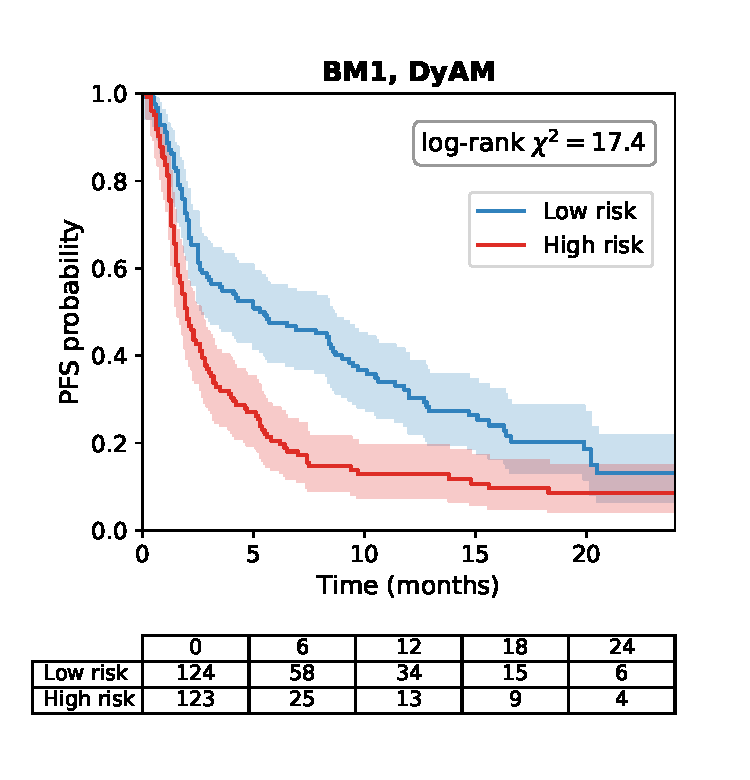
\includegraphics[width=0.48\textwidth]{figures/fig4a_km_bm1_dyam.pdf}}
  \hfill
  \subfloat[BM1, OvO]{%
    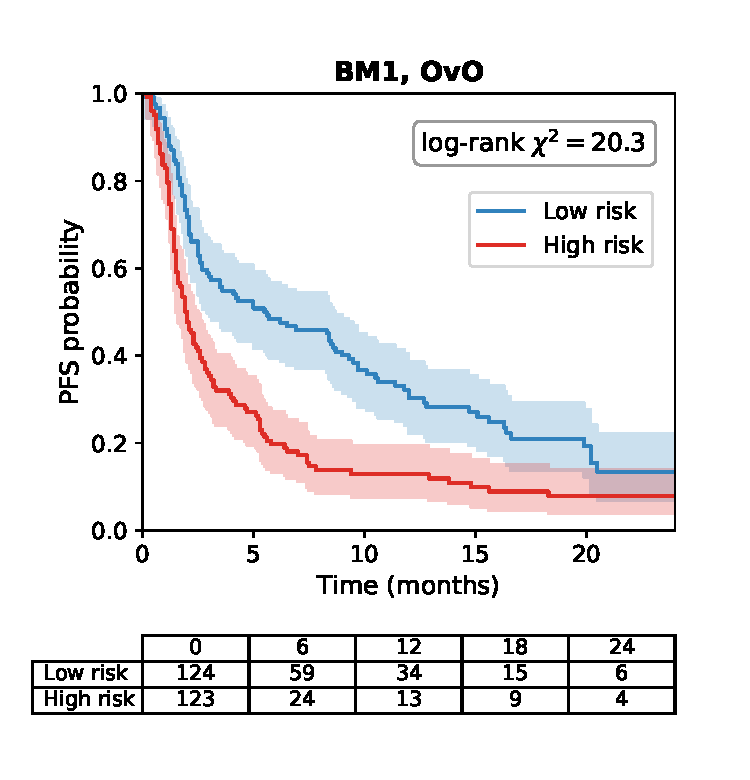
\includegraphics[width=0.48\textwidth]{figures/fig4b_km_bm1_ovo.pdf}}

  \subfloat[BM1, DyAM+NLP]{%
    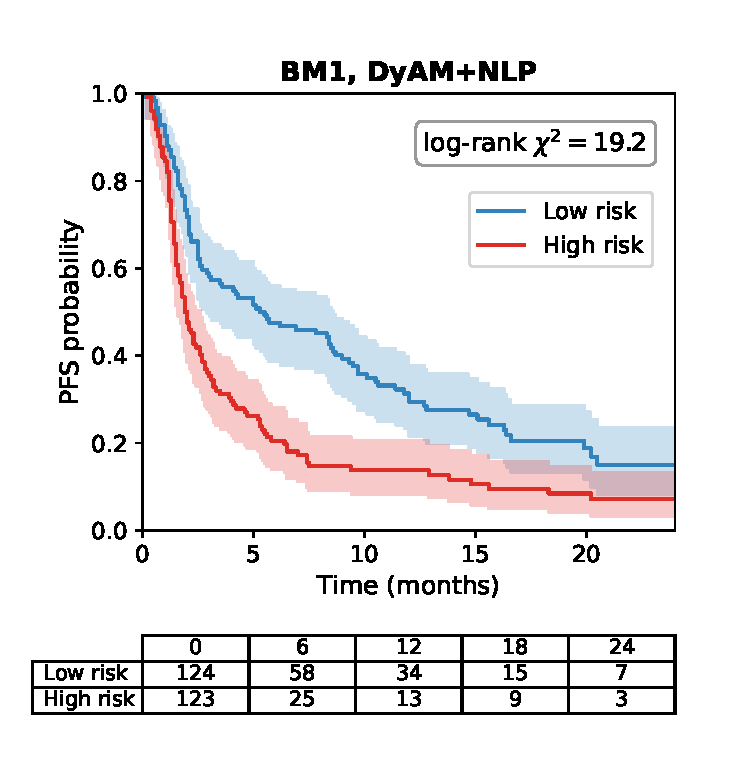
\includegraphics[width=0.48\textwidth]{figures/fig4c_km_bm1_dyam_nlp.pdf}}
  \hfill
  \subfloat[BM1, OvO+NLP]{%
    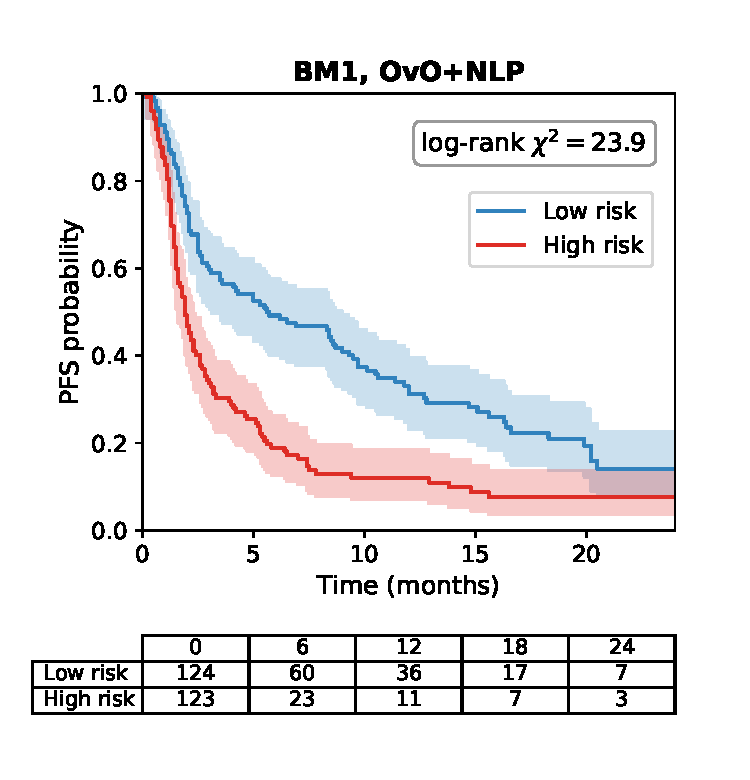
\includegraphics[width=0.48\textwidth]{figures/fig4d_km_bm1_ovo_nlp.pdf}}
  \caption{Kaplan--Meier progression-free survival curves at the primary benchmark BM1 (Rad+IHC-G+Gen+PDL1), computed from the out-of-fold risk
    scores of the single 10-fold partition and stratified at the median risk score into high-risk (red) and low-risk (blue) groups,
    with number-at-risk tables. The log-rank statistics printed in the panels are those of Table~\ref{tab:km} (BM1 rows;
    for the two +NLP panels the NLP encoding is added to the BM1 sources).
    (\textbf{A}) DyAM. (\textbf{B}) OvO. (\textbf{C}) DyAM+NLP. (\textbf{D}) OvO+NLP.}
  \label{fig:km_curves}
\end{figure}

\begin{figure}[H]
  \centering
  \subfloat[Harrell's C-index]{%
    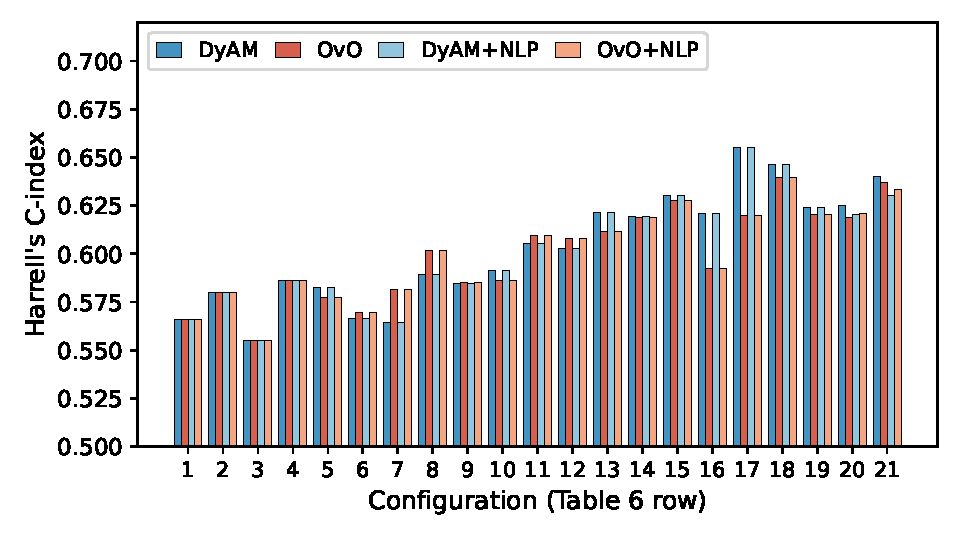
\includegraphics[width=0.48\textwidth]{figures/fig5a_cindex.pdf}}
  \hfill
  \subfloat[Time-dependent AUC at 12~months]{%
    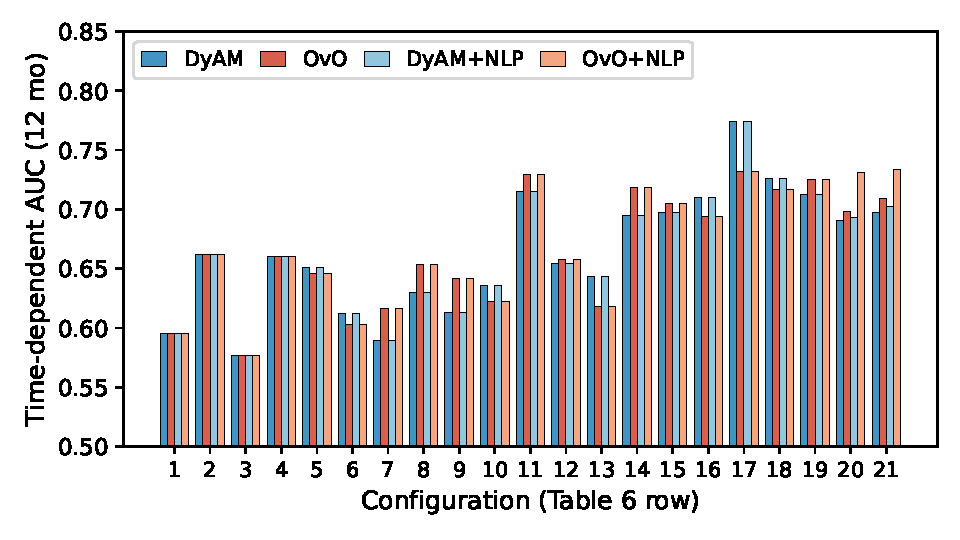
\includegraphics[width=0.48\textwidth]{figures/fig5b_tdauc.pdf}}

  \subfloat[Multivariate Cox hazard ratio]{%
    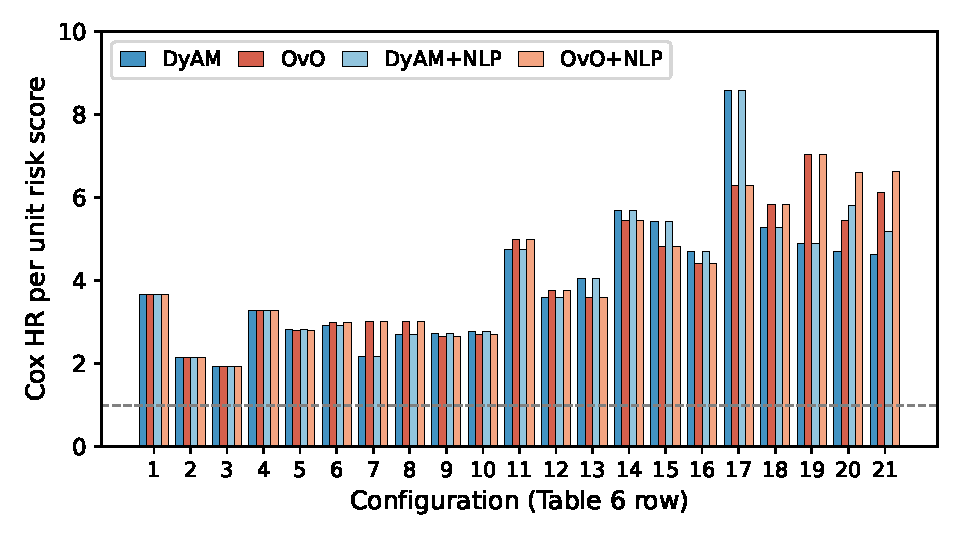
\includegraphics[width=0.48\textwidth]{figures/fig5c_cox_forest.pdf}}
  \hfill
  \subfloat[Kaplan--Meier log-rank $\chi^2$]{%
    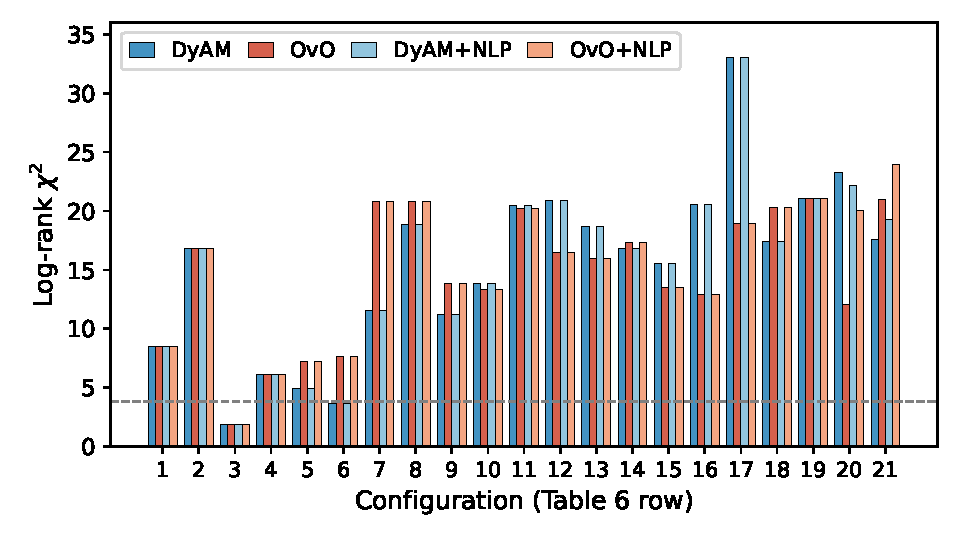
\includegraphics[width=0.48\textwidth]{figures/fig5d_km_chi2.pdf}}
  \caption{Survival association of the risk score across the 21 configurations (numbered as in Table~\ref{tab:ovo_all21}), single 10-fold partition.
    Bars show DyAM, OvO, and, where they differ (configurations 20 and 21), DyAM+NLP and OvO+NLP; for the other configurations the +NLP bars repeat the values without NLP.
    (\textbf{A}) Harrell's C-index (dashed line, 0.5).
    (\textbf{B}) Time-dependent AUC at 12 months.
    (\textbf{C}) Cox hazard ratio per unit of risk score, adjusted for age, ECOG performance status, albumin, dNLR and liver metastases (dashed line, 1).
    (\textbf{D}) Log-rank $\chi^2$ of the dichotomised risk score (dashed line, 3.84).}
  \label{fig:survival_summary}
\end{figure}

%% sections/discussion.tex — single-partition version
\section{Discussion}
\label{sec:discussion}

We extended the DyAM multimodal attention framework with two contributions, a competitive (OvO) attention
mechanism with fewer parameters and an NLP-based encoding of tabular clinical features, and evaluated them on
response (AUC) and progression-free survival in a 247-patient cohort using one 10-fold cross-validation partition.
The experiments support four conclusions.

\paragraph{Fusing sources is what moves performance.}
The best single sources reached AUCs of $0.708$ (PD-L1~TPS), $0.701$ (CT radiomics), $0.676$ (genomics) and $0.615$ (TMB).
Fusing four sources raised the AUC to $0.798$ under the cooperative attention of the original framework
($+0.090$ over PD-L1~TPS), a value that this evaluation reproduced and that matches the $0.80$ of the original
publication \cite{Vanguri2022}, and the best model reached $0.824$ (95\% CI $0.765$--$0.883$), $+0.116$ above
PD-L1~TPS, the biomarker in routine use, and above the modest discrimination reported for PD-L1 and TMB
\cite{Lu2019,Rizvi2015}.
The same pattern held for survival: the association of the risk score with progression-free survival rose
from a C-index of $0.56$--$0.59$ for a single source to $0.59$--$0.66$ for six or seven sources, and the log-rank
$\chi^2$ from $1.9$--$16.8$ to $12.1$--$33.0$. Two endpoints therefore point to the same
conclusion, that the sources carry complementary information that attention-based fusion can combine.

\paragraph{The NLP encoding of clinical variables is better than numeric labs.}
This was the most consistent finding of the study. Replacing the 13 numeric laboratory and clinical values by their
sentence embedding raised the AUC in all six comparisons that were made: $+0.018$ and $+0.019$ in the two pathology arms
under cooperative attention, $+0.019$ and $+0.022$ in the two seven-source configurations under cooperative attention, and
$+0.033$ and $+0.030$ in the same two configurations under OvO attention.
That a model that sees the encoded clinical profile in place of the numeric vector gains in every comparison, with both
attention mechanisms and both pathology encodings, makes a chance explanation less likely than a systematic benefit.
A plausible reason is that a sentence embedding represents combinations of variables, for example advanced age together
with low albumin and poor performance status, that are not explicit in a 13-dimensional numeric vector and that the
attention module would otherwise have to learn from a small training set \cite{Reimers2019,Wang2020MiniLM}; our data do
not test this mechanism.
The AUC with the encoding was also above that of the same sources without any clinical variable
($+0.020$ for DyAM and $+0.024$ for OvO at the primary benchmark), and the general-purpose sentence encoder was better than
the domain-specific BioClinBERT (Supplementary Note~S2), so no clinical fine-tuning was needed.

\paragraph{OvO attention gives the best fusion with a quarter of the parameters.}
At the primary benchmark OvO improved on cooperative attention by $+0.017$ without the NLP encoding ($0.801$ against $0.783$)
and by $+0.021$ with it ($0.824$ against $0.803$), and in the two seven-source configurations with labs OvO was above
the cooperative model as well ($0.782$ against $0.772$ and $0.824$ against $0.803$ with NLP).
OvO with the NLP encoding gave the highest AUC of all 21 configurations while training $1{,}242$ parameters against
$4{,}969$ for the cooperative model. OvO therefore offers the best accuracy of the two mechanisms with a simpler model;
the parameter count is a possible explanation, which we did not test by shrinking the cooperative attention matrix.
For survival, OvO with the NLP encoding gave the strongest separation of risk groups at BM2 (hazard ratio $6.64$
against $4.63$ for DyAM, log-rank $\chi^2 = 23.9$ against $17.6$, 12-month time-dependent AUC $0.733$ against $0.698$),
and the hazard ratio was higher for OvO at BM1 ($5.83$ against $5.27$), TMB+PDL1 ($3.00$ against $2.17$) and
Rad+IHC-A+Gen+TMB+PDL1 ($7.04$ against $4.88$). The C-index was close for the two mechanisms ($0.633$ against $0.640$ at BM2),
so the benefit of OvO lies in the separation of high- and low-risk groups rather than in the ranking of patients.
The cooperative model remained the stronger of the two in a few configurations, such as Rad+IHC-A+Gen+PDL1
($0.798$ against $0.768$), where it also had the strongest survival association of the study (C-index $0.655$, hazard ratio $8.59$),
so the choice between mechanisms may depend on the combination of sources.

\paragraph{The approach is practical.}
Encoding a patient profile takes less than one second on CPU, needs no labelled clinical text, and can be applied to any
structured electronic health record field that can be written as a sentence, so it can be transferred to other structured
clinical datasets without a fine-tuned clinical language model.

\paragraph{Clinical encodings and survival.}
The clinical encodings did not change the survival metrics consistently: hazard ratios were $5.0$--$6.3$, C-indices $0.62$--$0.64$ and
log-rank $\chi^2$ above $17$ for every variant. The NLP encoding matched numeric labs on these metrics, so its advantage in this study is on the
response endpoint, and we do not claim that it captures prognostic information.

\paragraph{Performance estimates.}
A harder evaluation gave lower values: training on the patients with the earliest CT accession numbers and testing on the later 124
(a proxy for time, since calendar dates were not available) gave AUCs of $0.703$ ($0.587$--$0.819$) for OvO+NLP and $0.700$ ($0.587$--$0.812$) for
DyAM+NLP, with $0.707$ and $0.678$ at seven sources. The cross-validated AUC of $0.824$ is therefore best read as the performance
under the evaluation protocol of the original framework rather than the expected performance in new patients. Because about 60 variants were compared on
the same 247 patients, the highest figures also include some selection, which we estimate at $0.014$--$0.031$ AUC.

\paragraph{Limitations.}
First, all results come from one 10-fold cross-validation partition of a single-institution retrospective cohort, which limits generalisability;
the confidence intervals reflect patient sampling but not the choice of partition.
Second, with $n = 247$ (62 responders) the 95\% interval of an AUC is about $\pm 0.07$, and the differences between models, which are
$0.02$ AUC or smaller, are smaller than this cohort can resolve (about 1{,}200--1{,}350 patients would be needed to detect $0.02$ AUC with 80\% power;
Supplementary Note~S3), so they are described by direction and magnitude.
Third, results depended on the numerical environment (the same code gave $0.798$ on Linux and $0.788$ on Windows at the primary benchmark), so all results
are from one pinned environment.
Fourth, the sentence encoder was used without fine-tuning on NSCLC clinical text.
Fifth, calendar dates were not available, so temporal validation was approximated by CT accession order and covered two configurations.
Finally, PD-L1 TPS was scored with the Sauter method, which may differ from the SP142 or 22C3 assays used elsewhere, so PD-L1-derived
features should be interpreted with this in mind.

%% sections/conclusion.tex — single-partition version
\section{Conclusions}
\label{sec:conclusion}

We extended the DyAM multimodal attention framework for ICI response prediction in NSCLC with a competitive (OvO)
attention mechanism and an NLP-based encoding of structured clinical variables, and the experiments
support four conclusions.
First, fusing sources is what raises performance: four fused sources reached an AUC of $0.798$ and the best model $0.824$
(95\% CI 0.765--0.883), against $0.708$ for PD-L1~TPS alone, and the association of the risk score with progression-free survival grew with the number of
fused sources across the 21 configurations (C-index up to $0.66$).
Second, the NLP encoding of clinical variables with a general-purpose sentence transformer exceeded numeric labs in all six comparisons
($+0.018$ and $+0.019$ in the two pathology arms, $+0.019$ to $+0.033$ in the two seven-source configurations), without any
fine-tuning on clinical text.
Third, OvO attention with the NLP encoding gave the highest AUC at the primary benchmark ($0.824$ against $0.803$ for cooperative
attention and $0.783$ for the original framework, $+0.041$) with about a quarter of the trainable parameters, and
the strongest separation of risk groups in the labs-replaced configuration of BM2 (hazard ratio $6.64$ against $4.63$,
log-rank $\chi^2 = 23.9$ against $17.6$, 12-month time-dependent AUC $0.733$ against $0.698$), although the C-index was similar ($0.633$ against $0.640$).
Fourth, the approach is practical, since encoding a patient takes less than one second on CPU and needs no labelled clinical text.
These results come from a single 10-fold partition, and an order-based hold-out evaluation gave lower estimates ($0.703$ for OvO+NLP and
$0.700$ for DyAM+NLP), so the cross-validated AUCs should not be read as expected performance in new patients.
Validation in larger, multi-institutional cohorts with calendar dates is needed to confirm these findings and to establish their
clinical utility for treatment selection.


%% ── MDPI mandatory back-matter declarations ─────────────────────────────────
\authorcontributions{%
  Conceptualization, methodology, software, formal analysis, investigation,
  writing---original draft preparation, and writing---review and editing, V.H.H.
  The author has read and agreed to the published version of the manuscript.
}

\dataavailability{%
  The code used in this study is available at
  \url{https://github.com/hoanghuyvu2k/Multimodal-Lung-Cancer}.
  Patient-level data are subject to institutional data-sharing agreements
  and available upon reasonable request.
}

\conflictsofinterest{The author declares no conflicts of interest.}

\bibliography{references}

\end{document}
